\chapter{一维基于紧致埃尔米特重构的双曲守恒律两步四阶数值格式}
\label{sec:1D-method}

在\cref{sec:framework}中,
我们为了使用紧致的埃尔米特重构,
提出了改进的两步四阶时间推进框架。
接下来,
我们将基于此框架设计一维的基于紧致埃尔米特重构的基本无振荡的两步四阶数值格式。
为此,
我们要选择适当的重构算法和解法器。

\section{广义黎曼问题解法器}
\label{sec:1D-solver-sec3}

在一维情形下,
本文采用Godunov解法器和文\cite{GRP}中的广义黎曼问题解法器作为标准一阶LW型解法器,
然后使用\cref{sec:1D-Solver}中的线性二阶LW型解法器。
下面我们以欧拉方程组为例,
简单介绍一下Godunov解法器和广义黎曼问题解法器。
为了方便表述,
本小节将$(x_{i+\frac{1}{2}},t^n)$平移到原点,
用符号$\bm u_L$、$\bm u_R$、$\bm u'_L$和$\bm u'_R$代替输入的四个值${\bm{u}}_{i+\frac{1}{2},-}^n$、${\bm{u}}_{i+\frac{1}{2},+}^n$、$\left({\partial_{x}}{\bm{u}}\right)_{i+\frac{1}{2},-}^n$和$\left({\partial_{x}}{\bm{u}}\right)_{i+\frac{1}{2},+}^n$,
用符号$\bm u_*$和$\left({\partial_t}\bm u\right)_*$代替需要输出的两个值${\bm u}_{i+\frac{1}{2}}^{n,+}$和$\left({\partial_{t}}{\bm{u}}\right)_{i+\frac{1}{2}}^{n,+}$。

\subsection{黎曼问题解法器:Godunov解法器}

两步四阶时间推进框架提供给解法器的输入是一个广义黎曼问题,
\begin{equation}
  \label{eq:1D-GRP}
  \left\{
  \begin{aligned}
     & {\partial_{t}}{\bm{u}} + {\partial_{x}}{\bm{f}}({\bm{u}}) = 0, \\
     & {\bm{u}}(x,0) =
    \begin{cases}
      \bm u_L + \bm u'_L x, & x<0,  \\
      \bm u_R + \bm u'_R x, & x>0.
    \end{cases}
  \end{aligned}
  \right.
\end{equation}
这个广义黎曼问题关联着一个黎曼问题:
\begin{equation}
  \label{eq:1D-RP}
  \left\{
  \begin{aligned}
     & {\partial_{t}}{\bm{u}^A} + {\partial_{x}}{\bm{f}}({\bm{u}^A}) = 0, \\
     & {\bm{u}^A}(x,0) =
    \begin{cases}
      \bm u_L, & x<0,  \\
      \bm u_R, & x>0.
    \end{cases}
  \end{aligned}
  \right.
\end{equation}
两者的一个典型的波系结构配置如\cref{fig:wave_pattern}。
假设${\bm u}(x,t)$是 \cref{eq:1D-GRP} 的解,
${\bm R}^A\left(x/t;\bm u_L,\bm u_R\right)$是 \cref{eq:1D-RP} 的解,
那么有时间渐近性定理\upcite{GRP_qi}
\begin{equation}
  \lim_{t\to 0,+} {\bm u}(\alpha t,t) = {\bm R}^A\left(\alpha;\bm u_L,\bm u_R\right), \quad \forall\alpha\in\mathbb{R}.
\end{equation}
特别需要注意的是,
我们有
\begin{equation}
  \bm u_* = \lim_{t\to 0,+} {\bm u}(0,t) = {\bm R}^A\left(0;\bm u_L,\bm u_R\right).
\end{equation}
至此,
我们就可以通过Godunov解法器确定${\bm R}^A\left(x/t;\bm u_L,\bm u_R\right)$,
进而得到$\bm u_*$。

\begin{figure}[htbp]
  \centering
  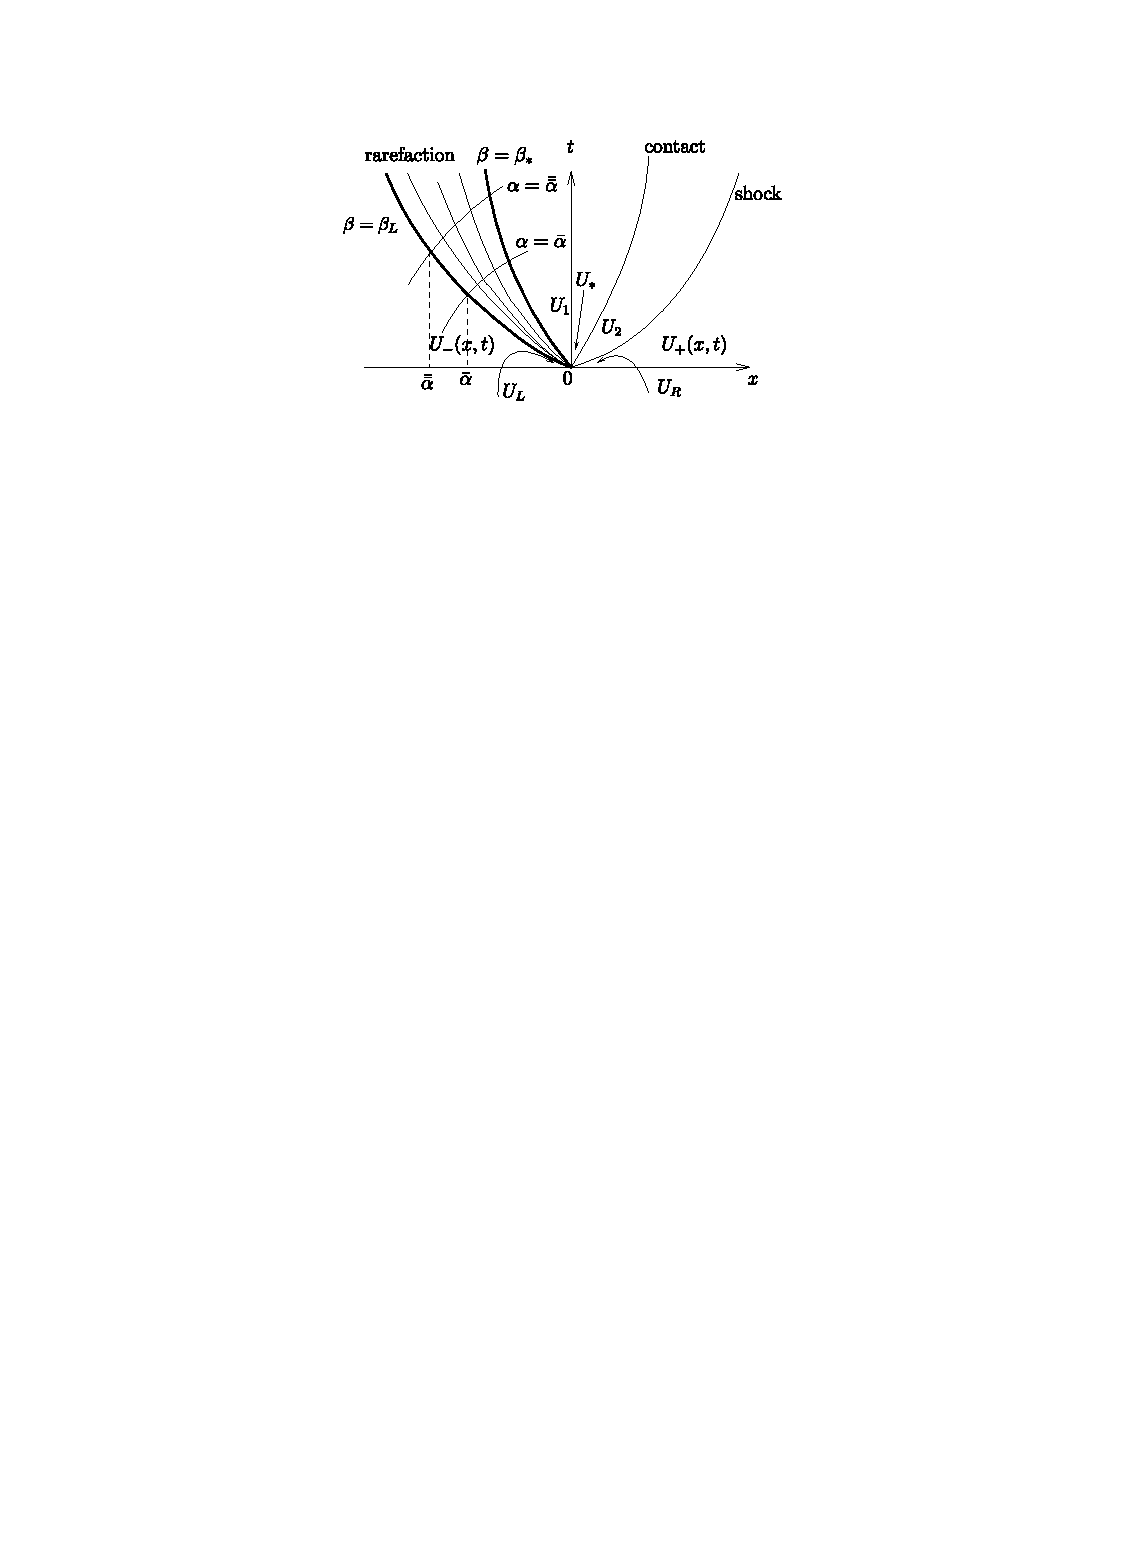
\includegraphics[width=0.8\textwidth]{fig/GRP_wave_pattern.pdf}
  \begin{center}(a)广义黎曼问题的波系结构\end{center}
  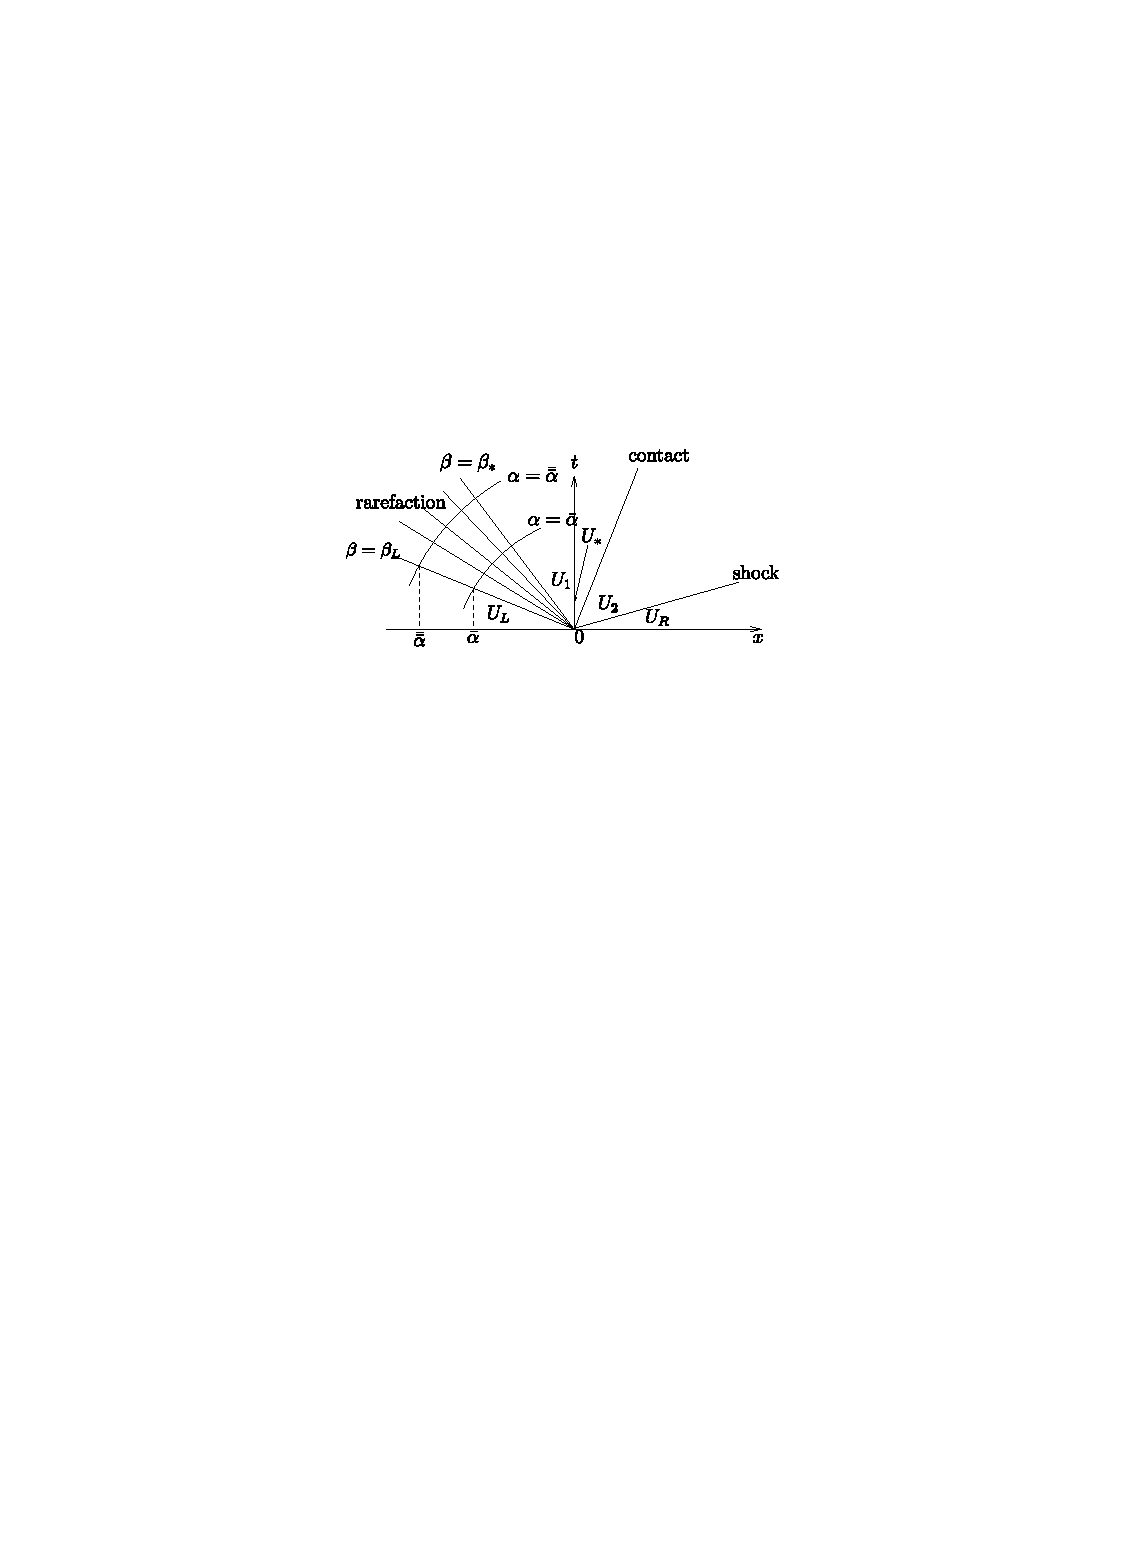
\includegraphics[width=0.8\textwidth]{fig/RP_wave_pattern.pdf}
  \begin{center}(b)相关联的黎曼问题的波系结构\end{center}
  \caption{一个典型的波系结构配置示意图。
    其中,
    1-波是稀疏波(rarefaction),
    2-波是接触间断(contact),
    以及3-波是激波(shock)。
  }
  \label{fig:wave_pattern}
\end{figure}

\subsection{线性声波近似的广义黎曼问题解法器}

文\cite{GRP}中介绍了两种广义黎曼问题解法器,
一种是精确求解的非线性解法器,
一种是线性声波近似的解法器。
在光滑处,
流场满足线性近似的声波方程,
采用声波近似的广义黎曼问题解法器;在间断附近则采用非线性的广义黎曼问题解法器。

接下来,
先介绍声波近似的广义黎曼问题解法器。
这种情形建立在流场光滑处,
即$\|\bm u_L-\bm u_R\|\ll 1$,
这一假设之上。
如果$t$轴位于$x$轴与1-波或3-波之间,
那么根据偏微分方程和解的连续性很容易求解$\left({\partial_t}\bm u\right)_*$。
这是一个平凡的情形,
故不再讨论。
其他情况,
可以通过下面的公式得到一阶导数
\begin{align}
   & \left({\partial_t}u\right)_* = -\frac{1}{2}\left(\left(u_*+c_*\right)\left(u'_L+\frac{p'_L}{\rho_*c_*}\right)+\left(u_*-c_*\right)\left(u'_R-\frac{p'_R}{\rho_*c_*}\right)\right),         \\
   & \left({\partial_t}p\right)_* = -\frac{\rho_*c_*}{2}\left(\left(u_*+c_*\right)\left(u'_L+\frac{p'_L}{\rho_*c_*}\right)-\left(u_*-c_*\right)\left(u'_R-\frac{p'_R}{\rho_*c_*}\right)\right), \\
   & \left({\partial_t}\rho\right)_* =
  \begin{cases}
    \frac{1}{c_*^2}\left(\left({\partial_t}p\right)_*+u_*\left(p'_L-c_*^2\rho'_L\right)\right), & u_* > 0,  \\
    \frac{1}{c_*^2}\left(\left({\partial_t}p\right)_*+u_*\left(p'_R-c_*^2\rho'_R\right)\right), & u_* > 0,
  \end{cases}
\end{align}
这里的公式仅针对欧拉方程组,
其中的$\rho$是密度,
$u$是速度,
$p$是压力,
$c$是声速。

\subsection{非线性广义黎曼问题解法器:\texorpdfstring{$t$}{t}轴不位于稀疏波内部}

下面我们简单介绍非线性的广义黎曼问题解法器。
出于同样的原因,
这里也不再讨论$t$轴位于$x$轴与1-波或3-波之间的平凡情形。
为了简便起见,
这里只介绍完全气体状态方程的结果,
一般状态方程的结果请参考文献\cite{GRP}。
这里先讨论$t$轴不位于稀疏波内部的情况。
一个关键点是跨越接触间断时,
$\left(\frac{Du}{Dt}\right)_*$和$\left(\frac{Dp}{Dt}\right)_*$的值是连续的,
其中$\frac{D}{Dt} = {\partial_t} + u_* {\partial_x}$是物质导数。

\vspace{0.3\baselineskip} % 自定义序列
{\noindent\bf 第一步:}建立非线性波两侧的关系。
在1-稀疏波两侧有
\begin{equation}
  \label{eq:1D-GRP-rare-guanxi}
  \begin{aligned}
     & a_L \left(\frac{Du}{Dt}\right)_* + b_L \left(\frac{Dp}{Dt}\right)_* = d_L, \quad a_L = 1, \quad b_L = \frac{1}{\rho_{2*}c_{2*}}, \\
     & d_L =
    \frac{T_Ls'_L}{1+2\mu^2} \left((1+\mu^2)\left(\frac{c_{2*}}{c_L}\right)^{1/(2\mu^2)}+\mu^2\left(\frac{c_{2*}}{c_L}\right)^{(1+\mu^2)/\mu^2}\right)-c_L\left(\frac{c_{2*}}{c_L}\right)^{1/(2\mu^2)}\psi'_L,
  \end{aligned}
\end{equation}
其中,
下标$2*$代表1-波和接触间断之间的状态,
可以通过黎曼问题解法器得到,
$T$是温度,
$s$是熵,
$\mu$是一个与多方指数$\gamma$有关的指数,
$\psi$是黎曼不变量之一,
以及它们可以由下式求得
\begin{equation}
  T_Ls'_L = \frac{p'_L-\rho'_Lc_L^2}{(\gamma-1)\rho_L}, \quad
  \mu = \sqrt{\frac{\gamma-1}{\gamma+1}}, \quad
  \psi'_L=u'_L+\left(\frac{\gamma p'_L}{c_L}-c_L\rho'_L\right) \frac{1}{(\gamma-1)\rho_L}.
\end{equation}
在3-稀疏波两侧也有类似的结果。
在3-激波两侧有
\begin{equation}
  \begin{aligned}
     & a_R \left(\frac{Du}{Dt}\right)_* + b_R \left(\frac{Dp}{Dt}\right)_* = d_R, \quad a_R = 1 + \rho_{3*}(\sigma-u_*) \mathcal{H}_1, \quad b_R = -\left(\frac{\sigma-u_*}{\rho_{3*}c_{3*}^2} + \mathcal{H}_1\right), \\
     & d_R = \left(-\frac{1}{\rho_R} + (\sigma-u_R) \mathcal{H}_2\right) p'_R + \left((\sigma-u_R) - \rho_R c_R^2 \mathcal{H}_2 - \rho_R \mathcal{H}_3\right) u'_R + \left((\sigma-u_R)\mathcal{H}_3\right) \rho'_R,
  \end{aligned}
\end{equation}
其中,
下标$3*$代表3-波和接触间断之间的状态,
也可以通过黎曼问题解法器得到,
$\sigma$代表间断速度,
以及
\begin{equation}
  \begin{aligned}
    \mathcal{H}_1 & = \frac{\mathcal{H}\left(p_*+(1+2\mu^2)p_R\right)}{2(p_*+\mu^2 p_R)},      & \quad
    \mathcal{H}_2 & = -\frac{\mathcal{H}\left((2+\mu^2)p_*+\mu^2p_R\right)}{2(p_*+\mu^2 p_R)},          \\
    \mathcal{H}_3 & = -\frac{\mathcal{H}\left(p_*-p_R\right)}{2\rho_R},                        & \quad
    \mathcal{H}   & = \sqrt{\frac{1-\mu^2}{\rho_R(p_*+\mu^2p_R)}}.
  \end{aligned}
\end{equation}
在1-激波两侧也有类似的结果。
总之,
无论1-波和3-波的组合情况如何,
我们都有
\begin{equation}
  \label{eq:1D-GRP-guanxi}
  \left\{
  \begin{aligned}
    a_L \left(\frac{Du}{Dt}\right)_* + b_L \left(\frac{Dp}{Dt}\right)_* & = d_L,  \\
    a_R \left(\frac{Du}{Dt}\right)_* + b_R \left(\frac{Dp}{Dt}\right)_* & = d_R.
  \end{aligned}
  \right.
\end{equation}
想了解更多有关建立欧拉方程组的非线性波两侧关系的详细细节,
请参考文献\cite{GRPpolytropic}。

{\noindent\bf 第二步:}确定广义黎曼解。
根据物质导数的定义,
我们有
\begin{equation}
  \label{eq:1D-GRP-DDt}
  \left(\frac{Du}{Dt}\right)_{*} = \left({\partial_t}u\right)_* - \frac{u_*}{\rho_* c_*^2} \left(\frac{Dp}{Dt}\right)_{*}, \quad
  \left(\frac{Dp}{Dt}\right)_{*} = \left({\partial_t}p\right)_* - \rho_* u_* \left(\frac{Du}{Dt}\right)_{*}.
\end{equation}
联立 \cref{eq:1D-GRP-guanxi,eq:1D-GRP-DDt},
我们可以得到$\left({\partial_t}u\right)_*$和$\left({\partial_t}p\right)_*$。
然后根据$t$轴的位置分类讨论,
如果$t$轴位于接触间断和1-稀疏波之间,
根据热力学关系式$dp = c^2 d\rho + \left( \frac{\partial p}{\partial s} \right)_\rho ds$,
有
\begin{equation}
  \label{eq:1D-GRP-solve-rho-1}
  \left({\partial_t}\rho\right)_* = \frac{1}{c_{2*}^2}\left(\left({\partial_t}p\right)_*+\rho_{2*}u_*\left(\frac{c_{2*}}{c_L}\right)^\frac{1+\mu^2}{\mu^2}\frac{p'_L-c_{2*}^2\rho'_L}{\rho_L}\right).
\end{equation}
如果$t$轴位于接触间断和3-激波之间,
根据兰金-雨贡纽(Rankine-Hugoniot,
R-H)条件有如下关系式成立
\begin{equation}
  \label{eq:1D-GRP-solve-rho-2}
  g_\rho^R \left({\partial_t}\rho\right)_* + g_p^R \left({\partial_t}p\right)_* + g_u^R \left({\partial_t}u\right)_* = u_* h_R,
\end{equation}
其中,
\begin{equation}
  \begin{aligned}
     & g_\rho^R = u_*-\sigma, \quad g_p^R = \frac{\sigma}{c_{3*}^2} - u_* \mathcal{J}_1, \quad g_u^R = u_* \rho_{3*} (\sigma-u_*) \mathcal{J}_1, \\
     & h_R = (\sigma - u_R) \mathcal{J}_2 p'_R + (\sigma - u_R) \mathcal{J}_3 \rho'_R - \rho_R(\mathcal{J}_2 c_R^2 + \mathcal{J}_3) u'_R,
  \end{aligned}
\end{equation}
以及$\mathcal{J}_1$、$\mathcal{J}_2$和$\mathcal{J}_3$是
\begin{equation}
  \mathcal{J}_1 = \frac{\rho_R p_R (1-\mu^4)}{\left(p_R + \mu^2 p_*\right)^2}, \quad \mathcal{J}_2 = \frac{\rho_R p_* (\mu^4-1)}{\left(p_R + \mu^2 p_*\right)^2}, \quad \mathcal{J}_3 = \frac{p_*+\mu^2 p_R}{p_R + \mu^2 p_*}.
\end{equation}
由 \cref{eq:1D-GRP-solve-rho-1} 或者 \cref{eq:1D-GRP-solve-rho-2} 很容易就可以得到$\left({\partial_t}\rho\right)_*$。
\vspace{0.3\baselineskip} % 自定义序列

\subsection{非线性广义黎曼问题解法器:\texorpdfstring{$t$}{t}轴位于稀疏波内部}

我们还有一种情形没有讨论,
就是$t$轴位于稀疏波内部。
假设是1-稀疏波内部,
类似 \cref{eq:1D-GRP-rare-guanxi},
我们可以得到
\begin{equation}
  \left(\frac{Du}{Dt}\right)_* + \frac{1}{\rho_*c_*} \left(\frac{Dp}{Dt}\right)_* = d_L,
\end{equation}
其中,
$d_L$和之前一样,
是已知的。
同时我们有
\begin{equation}
  \frac{Du}{Dt} + \frac{1}{\rho c}\frac{Dp}{Dt}
  = {\partial_t}u + u {\partial_x}u + \frac{1}{\rho c}{\partial_t}p + \frac{u}{\rho c}{\partial_x}p
  = \left({\partial_t}u + \frac{1}{\rho c}{\partial_t}p\right) - \frac{u}{c}\left(\frac{Du}{Dt} + \frac{1}{\rho c}\frac{Dp}{Dt}\right).
\end{equation}
由于黎曼解${\bm u}_*$所在的那条稀疏波内的特征线在原点的方向就是$t$轴,
即满足$u_*-c_*=0$,
所以从上式可以得到,
\begin{equation}
  \label{eq:1D-GRP-sonic-1}
  \left({\partial_t}u\right)_* + \frac{1}{\rho_* c_*}\left({\partial_t}p\right)_*
  = \frac{u_*+c_*}{c_*}\left(\left(\frac{Du}{Dt}\right)_* + \frac{1}{\rho_*c_*} \left(\frac{Dp}{Dt}\right)_*\right)
  = 2d_L.
\end{equation}
另外由于对$t$的导数就是沿着$t$轴的方向导数,
对于黎曼不变量$\phi$,
有
\begin{equation}
  \begin{aligned}
    \left({\partial_t}\phi\right)_{*} & =\left({\partial_t}\phi\right)_{*}+\left(u_{*}-c_{*}\right)\left({\partial_x}\phi\right)_{*}=T_*\left({\partial_x}s\right)_{*} = -\frac{T_*}{c_*}\left({\partial_t}s\right)_{*},
  \end{aligned}
\end{equation}
其中,
$T$是温度。
所以有,
\begin{equation}
  \label{eq:1D-GRP-sonic-2}
  \left({\partial_t}u\right)_{*}-\frac{1}{\rho_{*} c_{*}}\left({\partial_t}p\right)_{*}=\left({\partial_t}\phi\right)_{*}+\frac{T_*}{c_*}\left({\partial_t}s\right)_{*}=0.
\end{equation}
联立 \cref{eq:1D-GRP-sonic-1,eq:1D-GRP-sonic-2},
我们就可以得到$\left({\partial_t}u\right)_{*}$和$\left({\partial_t}p\right)_{*}$,
然后类似 \cref{eq:1D-GRP-solve-rho-1} 的做法,
可以得到
\begin{equation}
  \left({\partial_t}\rho\right)_* = \frac{1}{c_{*}^2}\left(\left({\partial_t}p\right)_*+\rho_{*}u_*\left(\frac{c_{*}}{c_L}\right)^\frac{1+\mu^2}{\mu^2}\frac{p'_L-c_*^2\rho'_L}{\rho_L}\right).
\end{equation}

\vspace{\baselineskip} % 节的总结
本节中,
我们介绍了一维情形下的Godunov解法器和广义黎曼问题解法器。
接下来为了设计一个两步四阶格式,
我们还需要选择适当的重构算法。

\section{线性紧致埃尔米特重构及其相应的两步四阶格式}
\label{sec:1D-linear-rec}

我们注意到,
如果如同文\cite{du2018hermite}中的两步四阶格式一样,
使用五阶的HWENO重构\upcite{Qiu-Shu-2004},
所得格式的只有四阶精度,
并且相比四阶重构,
计算开销更大、更不紧致。
为此我们拟设计一个更加紧致的四阶重构用于两步四阶格式。
本节将首先设计一维线性紧致埃尔米特重构。
为了设计出更加紧致的重构,
我们将使用$k$个单元构成的模板内所有单元内的两个信息——单元平均值和导数平均值。
这导致只能设计出偶数阶精度重构,
即$2k$阶重构。
当$k=2$时,
就是我们所期望构造的四阶重构。

给定一个函数$u(x)$,
定义函数$u(x)$及其导数$v(x)$在计算单元$I_{i}$上的平均值为
\begin{equation}
  \bar u_{i} = \frac {1}{h} \int_{I_{i}} u(x)dx, \quad
  \bar v_{i} = \frac {1}{h} \int_{I_{i}} v(x)dx = \frac{1}{h} (u(x_{i+\frac 12})-u(x_{i-\frac 12})), \quad
  i=1,\cdots, N,
\end{equation}
其中,
$I_{i}=[x_{i-\frac 12},x_{i+\frac 12}]$是大小为$h_i=x_{i+\frac 12}-x_{i-\frac 12}$的计算单元。
我们要在模板
\begin{equation}
  \label{eq:stencils}
  S^k_{r}(i) = \bigcup_{m=0}^{k-1} I_{i-r+m}, \quad
  r=0,1,\cdots, k-1, k\ge 1,
\end{equation}
上,
寻找埃尔米特重构多项式$p^r_i(x)$,
其中上标$r$表示依赖于模板$S^k_r(i)$,
是模板的偏移量。
为了简便起见,
采用均匀网格,
即$h_i\equiv h$。
值得强调的是,
本章的重构也适用于非均匀网格。
我们要得到的埃尔米特重构多项式应该在单元$I_{i}$内,
是对$u(x)$的$2k$阶精度的近似,
即
\begin{equation}
  {\partial_x^d}p^r_i(x) ={\partial_x^d} u(x) +\mathcal{O}(h^{2k-d}),\quad
  d=0,1,2.
\end{equation}
因此,
在单元边界处$x=x_{i\pm \frac 12}$,
重构值满足
\begin{equation}
  ({\partial_x^d} u)_{i\pm \frac 12,\mp}^r = {\partial_x^d}p^r_i(x_{i\pm \frac 12})={\partial_x^d} u(x_{i\pm\frac 12})+\mathcal{O}(h^{2k-d}),\quad
  d=0,1,2.
\end{equation}

\subsection{线性紧致埃尔米特重构的推导}

在文\cite{WENO}中给出了函数的重构与其原函数在单元边界上的插值之间的关系。
为了给出函数的埃尔米特重构插值与其原函数在单元边界上的埃尔米特插值的关系,
我们引入$u(x)$的原函数
\begin{equation}
  U(x)=\int^x_a u(\xi)d\xi,
\end{equation}
其中,
$a$是一个足够小的下界。
那么对$m=0,1,\cdots,k-1$,
我们有
\begin{equation}
  \label{eq:pri-val}
  U (x_{i+\frac 12-r+m})=U(x_{i-\frac 12-r})+h\sum_{\ell=i-r}^{i-r+m}\bar u_{\ell},\quad
  {\partial_x}U(x_{i+\frac 12-r+m})={\partial_x}U(x_{i-\frac 12-r})+h\sum_{\ell=i-r}^{i-r+m}\bar v_{\ell}.
\end{equation}
此时,
我们可以对这一系列点值$(U(x_{i-\frac12-r+m}),{\partial_x}U(x_{i-\frac12-r+m}))$,
$m=0,1,\cdots,k-1$,
用埃尔米特插值得到多项式$P^r_i(x)$来近似$U(x)$。
然后就得到了我们要找的重构多项式$p^r_i(x) = {\partial_x}P^r_i(x)$。
注意$U(x_{i-\frac 12-r})$的值在求导数的时候消失了,
但这里还有一个未知的值${\partial_x}U(x_{i-\frac 12-r})$等待确定。

为了确定未知的值${\partial_x}U(x_{i-\frac 12-r})$,
我们引入差商来表示插值多项式$P^r_i(x)$,
差商的定义可以参考数值分析教科书\cite{Kreiss-book}。
对于重节点的集合
\begin{equation}
  N_{r}(i) =\{x_{i-\frac 12-r}, x_{i-\frac 12-r}, \cdots, x_{i-\frac 12-r+k}, x_{i-\frac 12-r+k}\} , \ \ \ r=0, \cdots, k-1,
\end{equation}
我们有差商
\begin{equation}
  \label{eq:2_10}
  U[x_{\ell-\frac 12}] = U(x_{\ell-\frac 12}), \quad
  U[x_{\ell-\frac 12},x_{\ell-\frac 12}] = {\partial_x}U(x_{\ell-\frac 12}), \quad
  U[x_{\ell-\frac 12},x_{\ell+\frac 12}] = \bar u_{\ell}, \quad
  \cdots,
\end{equation}
其中,
$\ell = i-r+m$。
此时,
埃尔米特插值多项式$P^r_i(x)$可以表示为:
\begin{equation}
  P^r_i(x)={\widehat\sum}_{\ell=0}^{ k}U\left[x_{i-\frac 12-r}, \cdots, x_{i-\frac 12-r+\ell}\right]
  \widehat\prod_{m=0}^{\ell}\left(x-x_{i-\frac 12-r+m}\right),
\end{equation}
其中,
$\widehat\sum$代表重节点求和,
$\widehat\prod$代表重节点求积。
例如,
当$k=1$,
$r=0$时,
我们有
\begin{equation}
  \begin{aligned}
    P^0_{i}(x) =
     & U[x_{i-\frac 12}] + U[x_{i-\frac 12},x_{i-\frac 12}](x-x_{i-\frac 12}) + U[x_{i-\frac 12},x_{i-\frac 12},x_{i+\frac 12}](x-x_{i-\frac 12})^2 \\
     & + U[x_{i-\frac 12},x_{i-\frac 12},x_{i+\frac 12},x_{i+\frac 12}](x-x_{i-\frac 12})^2(x-x_{i+\frac 12}).
  \end{aligned}
\end{equation}

如同之前指出的,
$2k + 1$次多项式$P^r_i(x)$有一个多余的自由度${\partial_x}U(x_{i-\frac 12-r})$需要确定。
由于$p^r_i(x)$应该有$2k$个自由度$(\bar u_{i-r+m},\bar v_{i-r+m})$,
$m=0,\cdots, k-1$,
故$p^r_i(x)$应该是$2k-1$次多项式,
所以它的原函数$P^r_i(x)$应该是一个$2k$次多项式,
即$P^r_i(x)$的首项系数应该是零。
根据 \cref{eq:pri-val} 以及差商的定义,
多项式$P^r_i(x)$的首项系数是
\begin{equation}
  \label{eq:1Drec-leadingterm}
  U\left[x_{i-\frac 12-r}, x_{i-\frac 12-r}, \cdots, x_{i-\frac 12-r+k}, x_{i-\frac 12-r+k}\right]
  =\sigma {\partial_x}U(x_{i-\frac 12-r})+\sum_{m=0}^{k-1} \phi_{m} \bar{u}_{i-r+m}+ h \sum_{m=0}^{k-1} \psi_{m} \bar v_{i-r+m},
\end{equation}
当网格固定不变时,
其中的系数$\sigma$,
$\phi_m$和$\psi_m$是常数。
由于$P^r_i(x)$的首项系数应该是零,
即
\begin{equation}
  \label{eq:sigma_cal}
  \sigma {\partial_x}U(x_{i-\frac 12-r})+\sum_{m=0}^{k-1} \phi_{m} \bar{u}_{i-r+m}+h\sum_{m=0}^{k-1} \psi_{m} \bar v_{i-r+m} = 0.
\end{equation}
也就是说,
唯一待定的${\partial_x}U(x_{i-\frac 12-r})$可以从上式中解出。
一旦我们获得${\partial_x}U(x_{i-\frac 12-r})$,
我们就得到了插值多项式$P^r_i(x)$以及重构多项式$p^r_i(x)$。
需要指出的是,
我们还需要验证$\sigma\neq0$。

\begin{theorem}
  插值多项式$P^r_i(x)$的首项系数 \cref{eq:1Drec-leadingterm} 中的系数$\sigma$满足$\sigma\neq0$。
\end{theorem}
\begin{proof}
  由于$\sigma$与函数$U(x)$的取法无关,
  我们只需验证$\sigma$在一种特定的$U(x)$下满足条件即可。
  我们假设$U(x)$在节点集合$\{ x_{j-r-\frac 12},x_{j-r+\frac 12},\cdots,x_{j-r+k-\frac 12}\}$上满足$U(x)=0$,
  ${\partial_x}U(x)=1$。
  此时,
  有
  \begin{align}
     & \bar{u}_{i-r+m} = \frac{1}{h}\left(U(x_{i-r+m+\frac{1}{2}}) - U(x_{i-r+m-\frac{1}{2}})\right) = 0, \quad                        & m=0,\cdots,k-1,  \\
     & \bar v_{i-r+m} = \frac{1}{h}\left({\partial_x}U(x_{i-r+m+\frac{1}{2}}) - {\partial_x}U(x_{i-r+m-\frac{1}{2}})\right) = 0, \quad & m=0,\cdots,k-1.
  \end{align}
  所以,
  此时埃尔米特插值多项式$P(x)$的首项系数 \cref{eq:1Drec-leadingterm} 就是$\sigma$。
  
  接下来,
  我们考察$P(x)$的零点。
  首先,
  所有节点都是$P(x)$的零点,
  有$k+1$个。
  其次,
  由于${\partial_x}P(x_{j-r-\frac 12})=1>0$,
  存在$\xi_1>x_{j-r-\frac 12}$,
  使得对于$x\in [x_{j-r-\frac 12},\xi_1]$,
  有${\partial_x}P(x)>0$,
  进而有$P(\xi_1)>P(x_{j-r-\frac 12})=0$。
  类似地,
  因为${\partial_x}P(x_{j-r+\frac 12})=1>0$,
  所以存在$\xi_2\in(\xi_1,x_{j-r+\frac 12})$,
  使得对于$x\in [\xi_2,x_{j-r+\frac 12}]$,
  有${\partial_x}P(x)>0$,
  进而有$P(\xi_2)<P(x_{j-r+\frac 12})=0$。
  根据介值定理,
  存在$\xi\in[\xi_1,\xi_2]$,
  使得$P(\xi)=0$。
  因此,
  在这$k+1$个节点之间有$k$个零点。
  所以,
  $P(x)$总共有至少$2k+1$个零点。
  
  最后,
  因为$P(x)\in\mathcal{P}^{2k+1}$有至少$2k+1$个零点,
  并且存在一个点$\xi_1$使得$P(\xi_1) \neq 0$,
  所以$P(x)$的首项系数$\sigma$是非零的。
\end{proof}

最后,
我们要说明一点,
如果不是为了建立埃尔米特插值和埃尔米特重构之间的关系,
我们也可以通过解方程组得到同样的结果。
例如,
在模板$S^k_r(i)$上,
重构多项式$p^r_i(x)$应该满足
\begin{align}
  \label{eq:solve-system-1}
   & p^r_i(x) = \sum_{\ell=0}^{2k-1} C_\ell x^\ell,
   & C_\ell\in\mathcal{R},~x\in I_i,
  \\\label{eq:solve-system-2}
   & \frac {1}{h} \int_{I_{i-r+m}} p^r_i(x)dx = \bar u_{i-r+m}, \quad
   & m=0,\cdots, k-1,
  \\\label{eq:solve-system-3}
   & \frac {1}{h} \left(p^r_i(x_{i-r+m+\frac{1}{2}}) - p^r_i(x_{i-r+m-\frac{1}{2}})\right) = \bar v_{i-r+m}, \quad
   & m=0,\cdots, k-1.
\end{align}
将 \cref{eq:solve-system-1} 带入 \cref{eq:solve-system-2,eq:solve-system-3},
并求解得到的方程组,
可以得到系数$C_\ell$,
我们就可以得到重构多项式$p^r_i(x)$。
经过验证,
这种方法得到的重构多项式和利用埃尔米特插值得到的多项式是相同的。

\subsection{线性紧致埃尔米特重构的例子}

上一小节中,
我们对一般的含有$k$个单元的模板给出了线性埃尔米特重构多项式的推导。
本小节我们将具体讨论$k=1,2,3,4$的情形。
虽然我们只需要四阶重构,
但是为了工作的系统性,
在这里给出了从二阶到八阶精度的例子。

\subsubsection{$k=1$情形下的线性紧致埃尔米特重构}

当$k=1$且$r=0$时,
我们有
\begin{equation}
  \label{eq:1D-HC2}
  p^0_{i}(x) =p_{i}(x) = \bar u_{i} + \bar v_{i}(x-x_{i}), \quad
  {\partial_x}p_{i}(x)=\bar v_{i}, \quad
  x\in I_{i}.
\end{equation}
然后在单元$I_{i}$的边界处,
我们有
\begin{equation}
  u_{i+\frac 12,-} = \bar u_{i} + \frac{h}{2}\bar v_{i}, \quad
  u_{i-\frac 12,+} = \bar u_{i} - \frac{h}{2}\bar v_{i}, \quad
  ({\partial_x} u)_{i+\frac 12,-} = \bar v_{i}, \quad
  ({\partial_x} u)_{i-\frac 12,+} = \bar v_{i}.
\end{equation}
特别地,
我们规定
\begin{equation}
  ({\partial_x^2} u)_{i+\frac 12,-} = 0, \ \ \
  ({\partial_x^2} u)_{i-\frac 12,+} = 0.
\end{equation}
这种重构方法恰好是van Leer在文\cite{van-Leer}中的提出的二阶格式采用的重构。

\subsubsection{$k=2$情形下的线性紧致埃尔米特重构}

当$k=2$时,
有两个模板$S^2_0(i)$(对应$r=0$)以及$S^2_1(i)$(对应$r=1$)。
在$S^2_0(i)$上,
我们可以写出多项式$P^0_{i}(x)$:
\begin{equation}
  \begin{aligned}
    P^0_{i}(x) =
     & U[x_{i-\frac 12}] + U[x_{i-\frac 12},x_{i-\frac 12}](x-x_{i-\frac 12}) + U[x_{i-\frac 12},x_{i-\frac 12},x_{i+\frac 12}](x-x_{i-\frac 12})^2                        \\
     & + U[x_{i-\frac 12},x_{i-\frac 12},x_{i+\frac 12},x_{i+\frac 12}](x-x_{i-\frac 12})^2(x-x_{i+\frac 12})                                                              \\
     & + U[x_{i-\frac 12},x_{i-\frac 12},x_{i+\frac 12},x_{i+\frac 12},x_{i+\frac{3}{2}}](x-x_{i-\frac 12})^2(x-x_{i+\frac 12})^2                                          \\
     & + U[x_{i-\frac 12},x_{i-\frac 12},x_{i+\frac 12},x_{i+\frac 12},x_{i+\frac{3}{2}},x_{i+\frac{3}{2}}](x-x_{i-\frac 12})^2(x-x_{i+\frac 12})^2(x-x_{i+\frac{3}{2}}),
  \end{aligned}
\end{equation}
此时$p^0_{i}(x)={\partial_x}P^0_{i}(x)$变成了
\begin{equation}
  \label{eq:HC-2}
  \begin{aligned}
    p^0_{i}(x)
     & = U[x_{i-\frac 12},x_{i-\frac 12}] + U[x_{i-\frac 12},x_{i-\frac 12},x_{i+\frac 12}]\xi_1 + U[x_{i-\frac 12},x_{i-\frac 12},x_{i+\frac 12},x_{i+\frac 12}]\xi_2 \\
     & + U[x_{i-\frac 12},x_{i-\frac 12},x_{i+\frac 12},x_{i+\frac 12},x_{i+\frac{3}{2}}]\xi_3,
  \end{aligned}
\end{equation}
其中$\xi_i(x)$,
$i=1,2,3$是
\begin{align}
   & \xi_1(x) = 2(x-x_{i-\frac 12}),                                                    \\
   & \xi_2(x) = (x-x_{i-\frac 12})(3x-2x_{i+\frac 12}-x_{i-\frac 12}),                  \\
   & \xi_3(x)=2(x-x_{i-\frac 12})(x-x_{i+\frac 12})(2x-x_{i+\frac 12}-x_{i-\frac 12}).
\end{align}
$U[x_{i-\frac 12},x_{i-\frac 12}] = {\partial_x}U(x_{i-\frac 12})$的值,
可以通过求解 \cref{eq:sigma_cal} 得到,
具体地说,
通过求解下面这个方程得到
\begin{equation}
  U[x_{i-\frac 12},x_{i-\frac 12},x_{i+\frac 12},x_{i+\frac 12},x_{i+\frac 32},x_{i+\frac{3}{2}}] = 0.
\end{equation}
因此,
我们可以得到$p^0_{i}(x)$的显式表达式,
并在单元$I_{i}$的边界$x=x_{i\pm \frac 12}$上得到
\begin{equation}
  ({\partial_x^d} u)_{i\pm1 / 2,\mp}^0 = {\partial_x^d} p^0_{i}(x_{i\pm1/2}), \quad d=0,1,2.
\end{equation}

类似的,
我们可以得到模板$S^2_1(i)$上的重构多项式$p^{1}_{i}(x)$,
以及$({\partial_x^d} u)_{i\pm1 / 2,\mp}^1$。

\subsubsection{均匀网格情况下线性紧致埃尔米特重构多项式的系数}

$k=3,4$的情形就不再具体讨论。
一旦我们给定了$k \ge 1$和$r$,
那么模板$S^k_r(i)$的选择就确定了,
如果我们知道了每个单元上的两个平均值$(\bar u_{i-r+m},\bar v_{i-r+m})$,
我们就可以得到$p^r_i(x)$。
然后在$x_{i\pm\frac 12}$处,
我们有以下形式的单元边界值
\begin{equation}
  \label{eq:Con}
  ({\partial_x^d} u)_{i\pm \frac 12,\mp}^{r} = \frac{1}{h^d}\sum_{m=0}^{k-1} \phi_{m,\mp}^{r,d} \bar{u}_{i-r+m}+ \frac{1}{h^{d-1}}\sum_{m=0}^{k-1} \psi_{m,\mp}^{r,d} \bar v_{i-r+m},\quad d=0,1,2,
\end{equation}
其中系数$\phi^{r,d}_{m,\mp}$和$\psi^{r,d}_{m,\mp}$在均匀网格的情况下是常数。
由于模板的对称性,
对于$m,r=0,1,\cdots,k-1$和$d=0,1,2$,
有
\begin{equation}
  \label{eq:co-re}
  \phi_{k-1-m,+}^{k-1-r,d} = (-1)^d \phi_{m,-}^{r,d},
  \quad \psi_{k-1-m,+}^{k-1-r,d} = (-1)^{d+1} \psi_{m,-}^{r,d}.
\end{equation}

在\cref{ta:Con} 中给出了在本章中使用的重构在均匀网格的情况下的系数$\phi^{r,d}_{m,-}$和$\psi^{r,d}_{m,-}$,
$d=0,1,2$,
而与其对称的模板的系数$\phi^{k-1-r,d}_{k-1-m,+}$和$\psi^{k-1-r,d}_{k-1-m,+}$可以根据 \cref{eq:co-re} 得到。

\begin{table}[htbp]
  \caption{在均匀网格的情况下,
    系数$\phi_{m,-}^{r,d}$和$\psi_{m,-}^{r,d}$,
    $k \le 4$。
  }
  \label{ta:Con}
  \centering
  \begin{tabular}{ccc cccc cccc}
    \toprule
    $k$ & $r$ & $d$ & $\phi_{0,-}^{r,d}$ & $\phi_{1,-}^{r,d}$ & $\phi_{2,-}^{r,d}$ & $\phi_{3,-}^{r,d}$ & $\psi_{0,-}^{r,d}$ & $\psi_{1,-}^{r,d}$ & $\psi_{2,-}^{r,d}$ & $\psi_{3,-}^{r,d}$ \\
    \midrule
    1   & 0   & 0   & 1                  & ~                  & ~                  & ~                  & 1/2                & ~                  & ~                  & ~                  \\
    1   & 0   & 1   & 0                  & ~                  & ~                  & ~                  & 1                  & ~                  & ~                  & ~                  \\
    1   & 0   & 2   & 0                  & ~                  & ~                  & ~                  & 0                  & ~                  & ~                  & ~                  \\
    2   & 0   & 0   & 1/2                & 1/2                & ~                  & ~                  & 1/6                & -1/6               & ~                  & ~                  \\
    2   & 0   & 1   & -2                 & 2                  & ~                  & ~                  & -1/2               & -1/2               & ~                  & ~                  \\
    2   & 0   & 2   & 0                  & 0                  & ~                  & ~                  & -1                 & 1                  & ~                  & ~                  \\
    3   & 1   & 0   & 11/60              & 19/30              & 11/60              & ~                  & 1/20               & 1/2                & -1/20              & ~                  \\
    3   & 1   & 1   & 1/4                & -2                 & 7/4                & ~                  & 1/12               & -1/6               & -5/12              & ~                  \\
    3   & 1   & 2   & -11/4              & -2                 & 19/4               & ~                  & -3/4               & -6                 & -3/4               & ~                  \\
    4   & 1   & 0   & 5/84               & 37/84              & 37/84              & 5/84               & 1/70               & 17/70              & -17/70             & -1/70              \\
    4   & 1   & 1   & -7/54              & -5/2               & 5/2                & 7/54               & -1/36              & -11/12             & -11/12             & -1/36              \\
    4   & 1   & 2   & -1                 & 1                  & 1                  & -1                 & -1/4               & -9/4               & 9/4                & 1/4                \\
    \bottomrule
  \end{tabular}
\end{table}

\subsection{基于线性紧致埃尔米特重构的两步四阶格式及其稳定性分析}

在上一小节,
我们已经得到了$k=1,2,3,4$下的十个线性紧致埃尔米特重构,
接下来我们要设计相应的格式,
并考察其线性稳定性。

$k=1$的二阶重构其实就是文\cite{Book-Matania}中的广义黎曼问题格式所用的重构。
这个重构是二阶的,
不适用于两步四阶时间推进。
对于$k=2,3,4$的九个线性重构,
使用我们在\cref{sec:1D-S2O4}中提出的改进的两步四阶时间推进框架,
其中的重构$\mathcal{R}$采用新设计的线性重构,
LW型解法器$\mathcal{G}$采用\cref{sec:1D-solver-sec3}中介绍的Godunov解法器和广义黎曼问题解法器。
然后,
我们得到了九个两步四阶格式。

接下来,
我们考察这九个数值格式的线性稳定性。
线性耗散分析有助于理解格式的稳定性,
选取线性对流方程
\begin{equation}
  \label{eq:linear}
  \dfrac{\partial u}{\partial t} +\widetilde{C}\dfrac{\partial u}{\partial x}=0, \quad \widetilde{C}=1,
\end{equation}
作为模型方程。
由于上一小节给出的九个数值格式属于双值格式,
即单元平均值$\bar u_{i}^n$和导数平均值$\bar v_{i}^n$同时被推进。
耗散性质应该从这两个分量的角度进行研究。
因此,
我们考虑以下傅立叶模式:
\begin{equation}
  \label{eq:Fourier}
  \bar u_{i}^n = \lambda^n e^{j\kappa ih}, \quad
  h \bar v_{i}^n = j\kappa h \mu^n e^{j\kappa ih}, \quad
  \kappa h \in [0,2\pi], \quad j^2=-1,
\end{equation}
其中$\lambda$和$\mu$是增长因子,
为了避免与一维的单元下标$i$混淆,
使用$j$作为虚数单位。
请注意,
$\lambda$和$\mu$并不相同,
因为单元平均值和导数平均值是通过不同的数值公式更新的。
数值格式的形式可以写成
\begin{align}
  \label{eq:f-2}
  \bar u_{i}^{n+1}   & = \sum_m a_m(\eta) \bar u_{i+m}^n + h\sum_m b_m(\eta) \bar v_{i+m}^n,  \\
  \label{eq:f-3}
  h \bar v_{i}^{n+1} & = \sum_m c_m(\eta) \bar u_{i+m}^n + h\sum_m d_m(\eta) \bar v_{i+m}^n.
\end{align}
其中,
$\eta=\tau / h$是时间步长和网格大小的比值,
$a_m$,
$b_m$,
$c_m$和$d_m$是依赖于特定数值格式的系数。
将 \cref{eq:Fourier} 带入 \cref{eq:f-2,eq:f-3},
得到
\begin{equation}
  \begin{bmatrix} \bar u_{i}^{n+1} \\[6mm]
    h \bar v_{i}^{n+1}\end{bmatrix}
  = \begin{bmatrix}
    \displaystyle \sum_m a_m(\eta) e^{j\kappa mh} & \displaystyle \sum_m b_m(\eta) e^{j\kappa mh} \\
    \displaystyle \sum_m c_m(\eta) e^{j\kappa mh} & \displaystyle \sum_m d_m(\eta) e^{j\kappa mh}
  \end{bmatrix}
  \begin{bmatrix} \bar u_{i}^{n} \\[6mm]
    h \bar v_{i}^{n}\end{bmatrix},
\end{equation}
接下来,
我们需要分析下面这个矩阵的谱半径,
\begin{equation}
  G=
  \begin{bmatrix}
    \displaystyle \sum_m a_m(\eta) e^{j\kappa mh} & \displaystyle \sum_m b_m(\eta) e^{j\kappa mh} \\
    \displaystyle \sum_m c_m(\eta) e^{j\kappa mh} & \displaystyle \sum_m d_m(\eta) e^{j\kappa mh}
  \end{bmatrix}.
\end{equation}
设$\rho_m$,
$m=1,2$是矩阵$G$的特征值,
那么$\rho_m(G)$的最大模就决定了数值格式的稳定性,
格式稳定的必要条件是
\begin{equation}
  \label{eq:stability-condition}
  \max_{m=1,2,~\kappa h\in[0,2\pi]} |\rho_m(G)|\le 1+\mathcal{O}(\tau).
\end{equation}

我们现在对得到的九个两步四阶格式,
分别进行如上所述的傅立叶分析,
得到了如\cref{fig:eigens-1,fig:eigens-2,fig:eigens-3,fig:eigens-4,fig:eigens-5} 的结果。
图中展示了两个特征值$\rho_m(G)$在复平面上的图像,
其中,
$\kappa h\in[0,2\pi]$,
$\eta = 0.6$。

\begin{figure}[htbp]
  \centering
  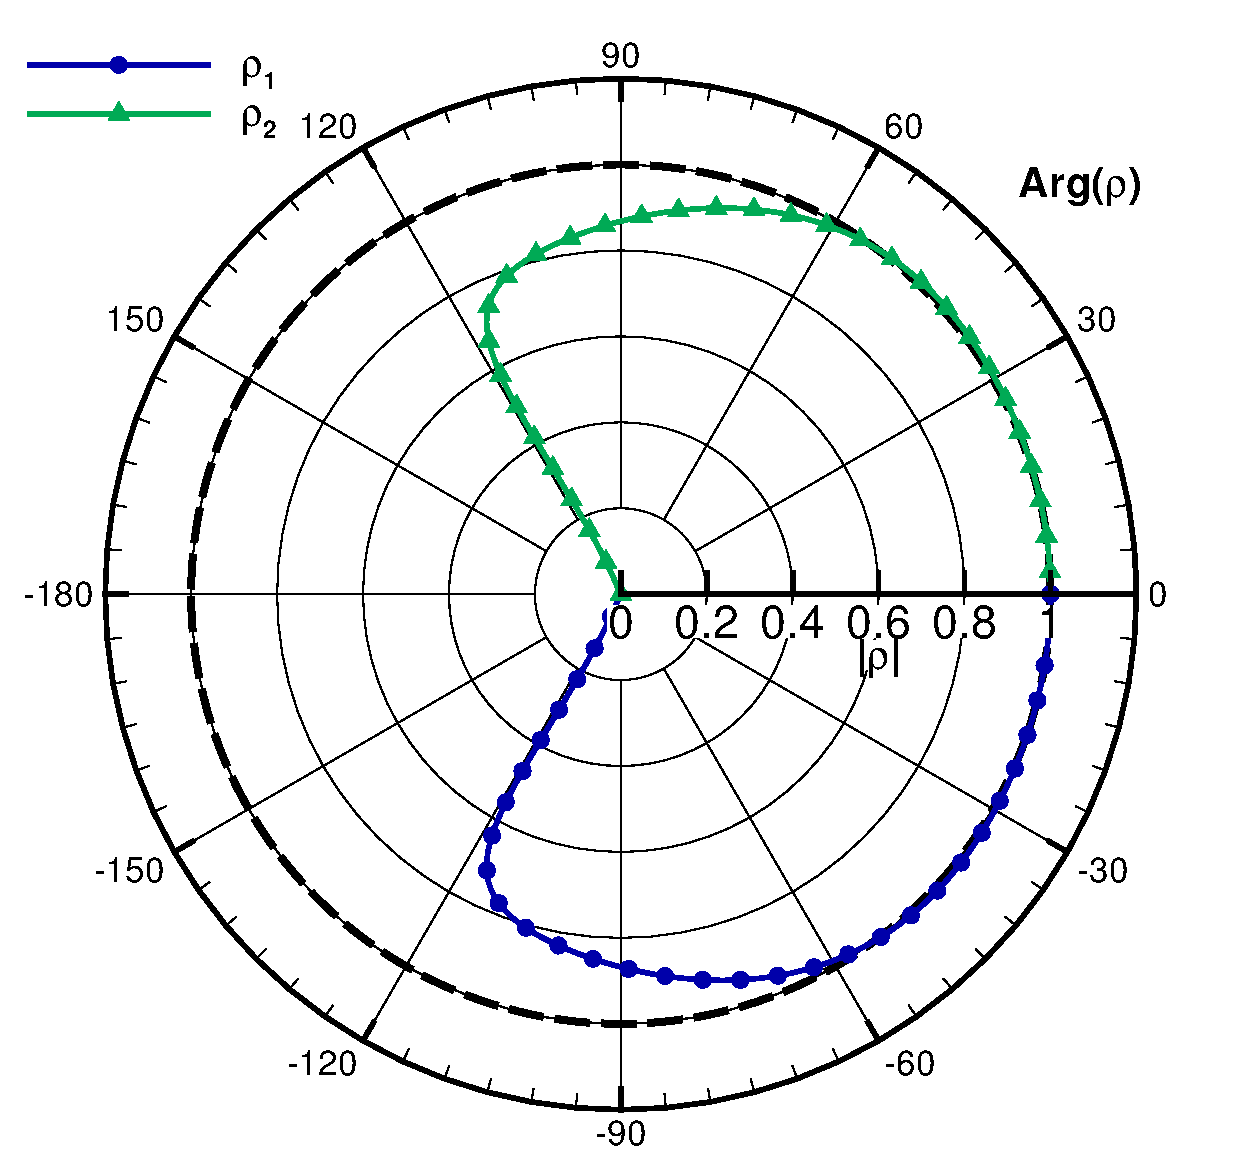
\includegraphics[width=0.74\textwidth]{fig/1D/pol40.pdf}
  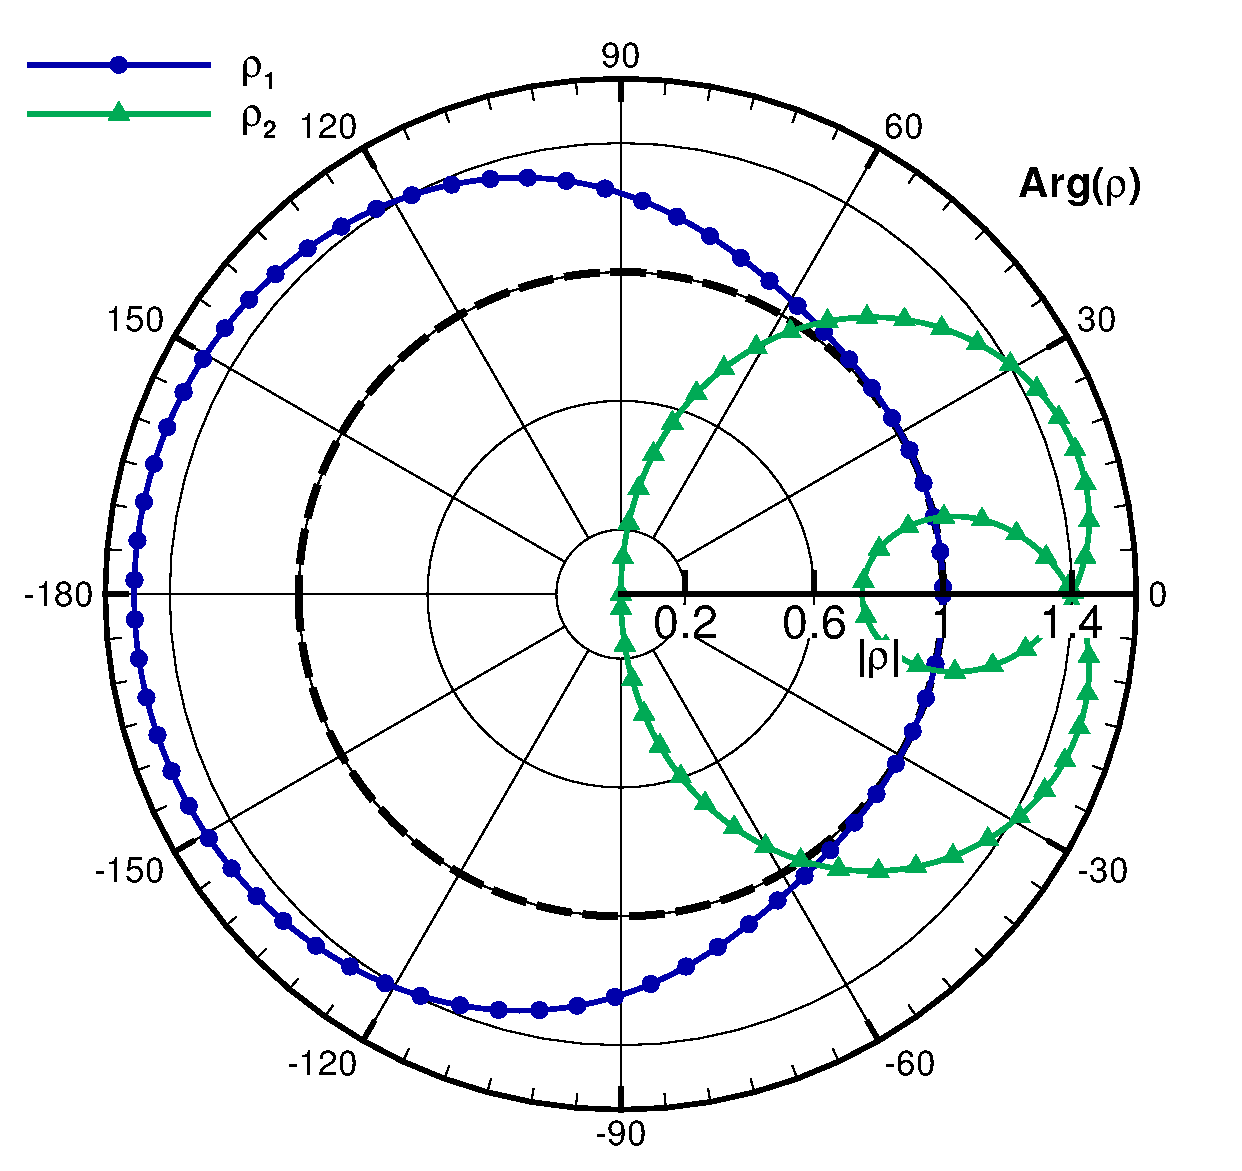
\includegraphics[width=0.74\textwidth]{fig/1D/pol41.pdf}
  \caption{$\rho_m(G)$在复平面的值。
    上:$k=2$,
    $r=0$,
    下:$k=2$,
    $r=1$。
    $k$是模板含有的单元数,
    $r$是 \cref{eq:stencils} 中定义的模板的偏移量,
    $\kappa h\in [0,2\pi]$,
    蓝色和绿色的线分别对应特征值$\rho_1(G)$和$\rho_2(G)$。
  }
  \label{fig:eigens-1}
\end{figure}

\begin{figure}[htbp]
  \centering
  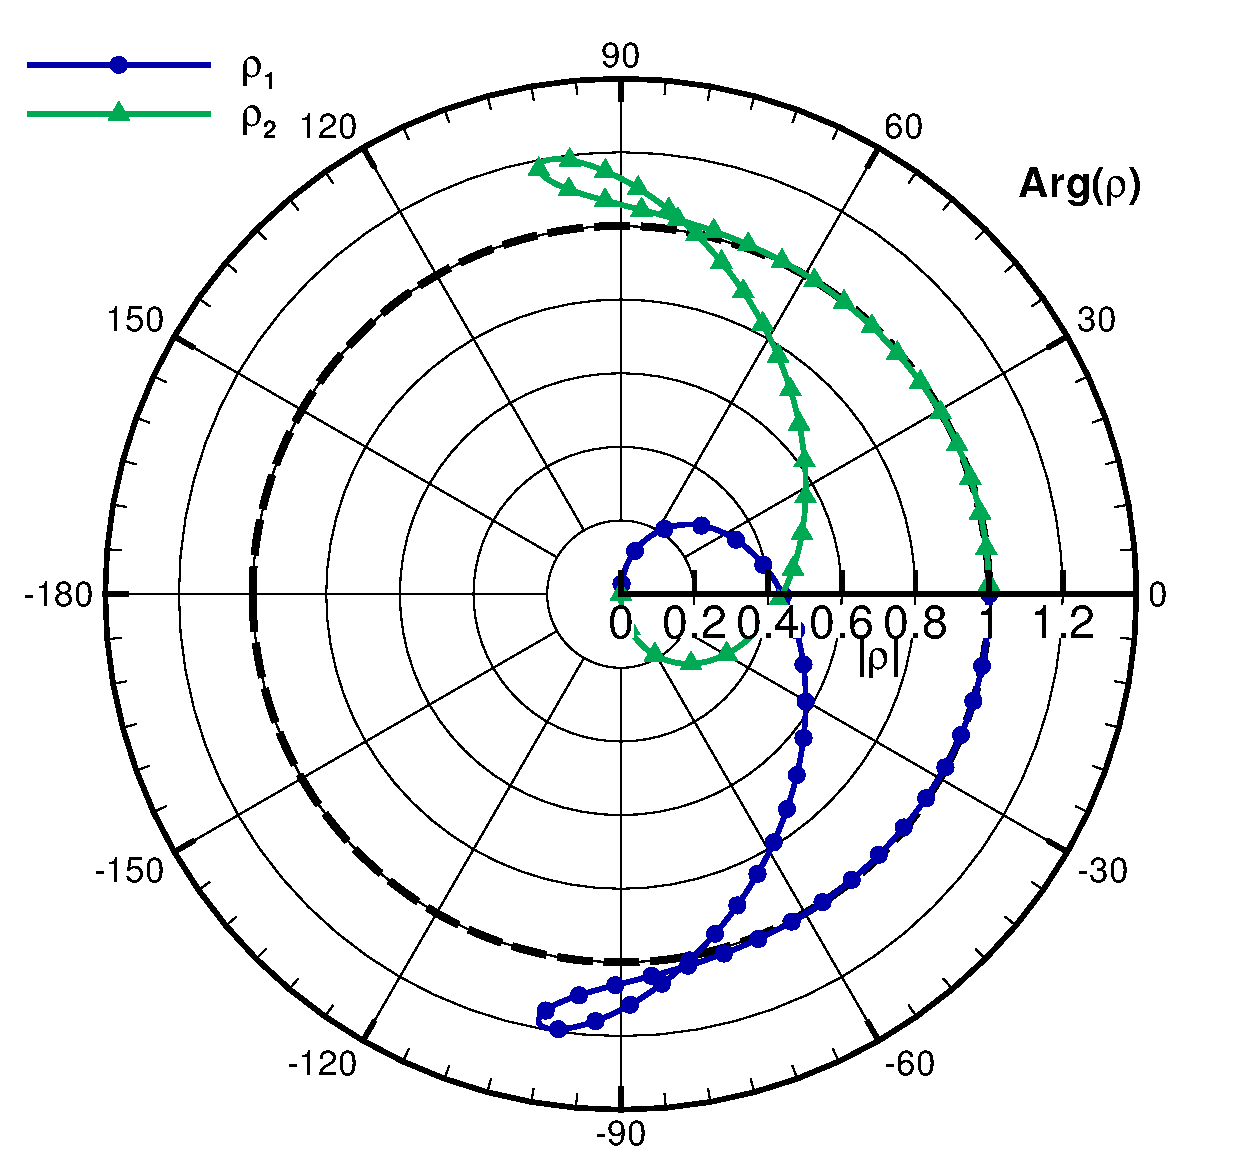
\includegraphics[width=0.74\textwidth]{fig/1D/pol60.pdf}
  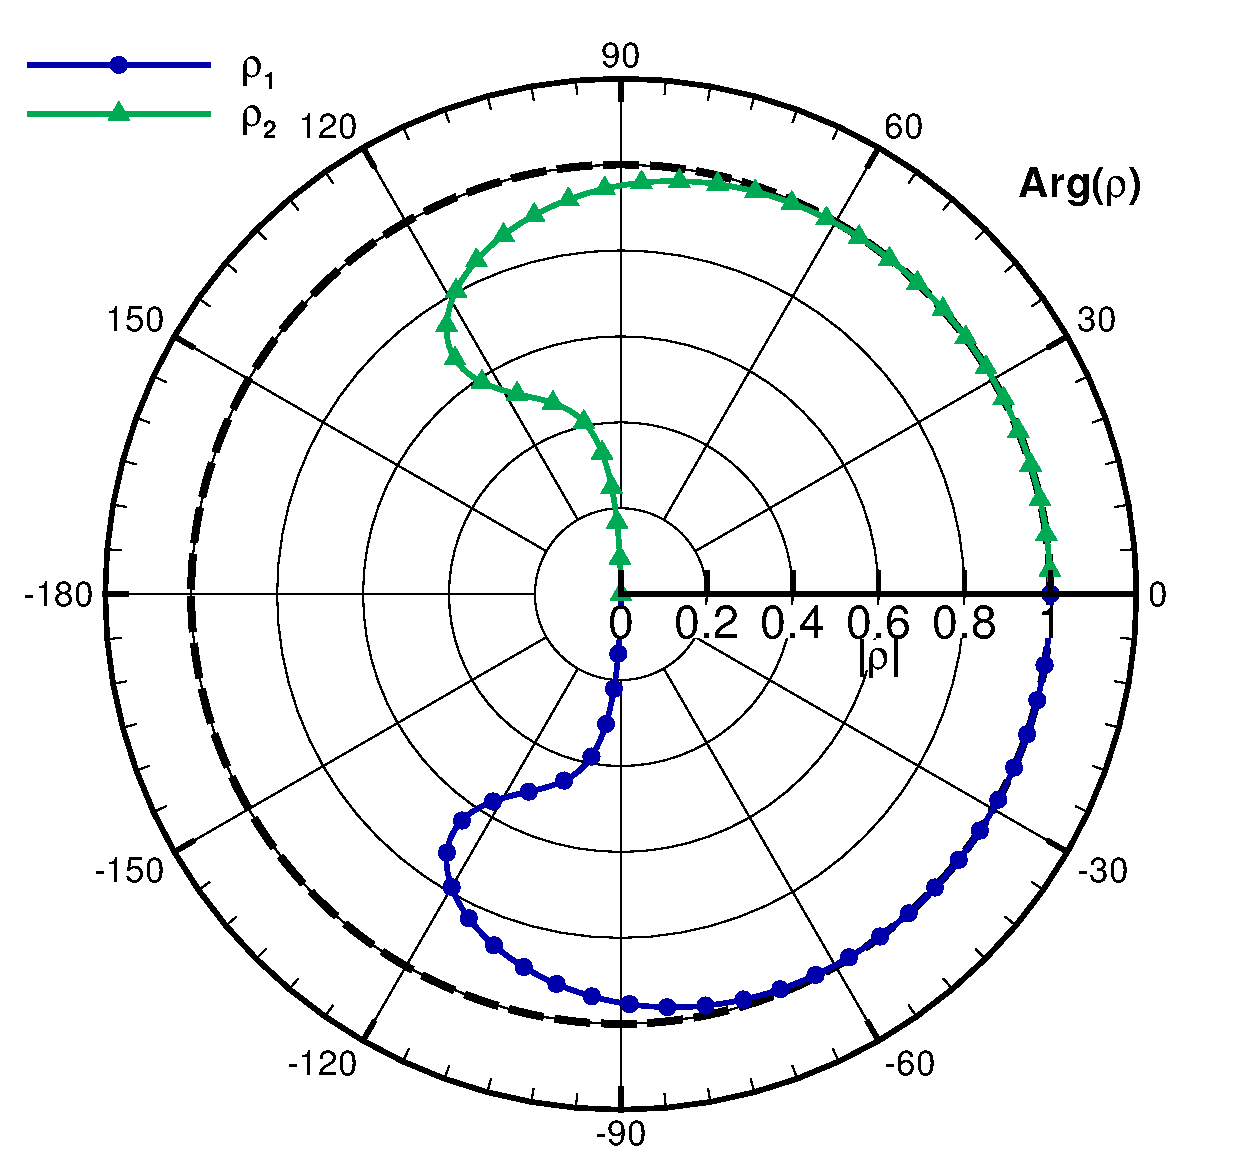
\includegraphics[width=0.74\textwidth]{fig/1D/pol61.pdf}
  \caption{$\rho_m(G)$在复平面的值。
    上:$k=3$,
    $r=0$,
    下:$k=3$,
    $r=1$。
    $k$是模板含有的单元数,
    $r$是 \cref{eq:stencils} 中定义的模板的偏移量,
    $\kappa h\in [0,2\pi]$,
    蓝色和绿色的线分别对应特征值$\rho_1(G)$和$\rho_2(G)$。
  }
  \label{fig:eigens-2}
\end{figure}

\begin{figure}[htbp]
  \centering
  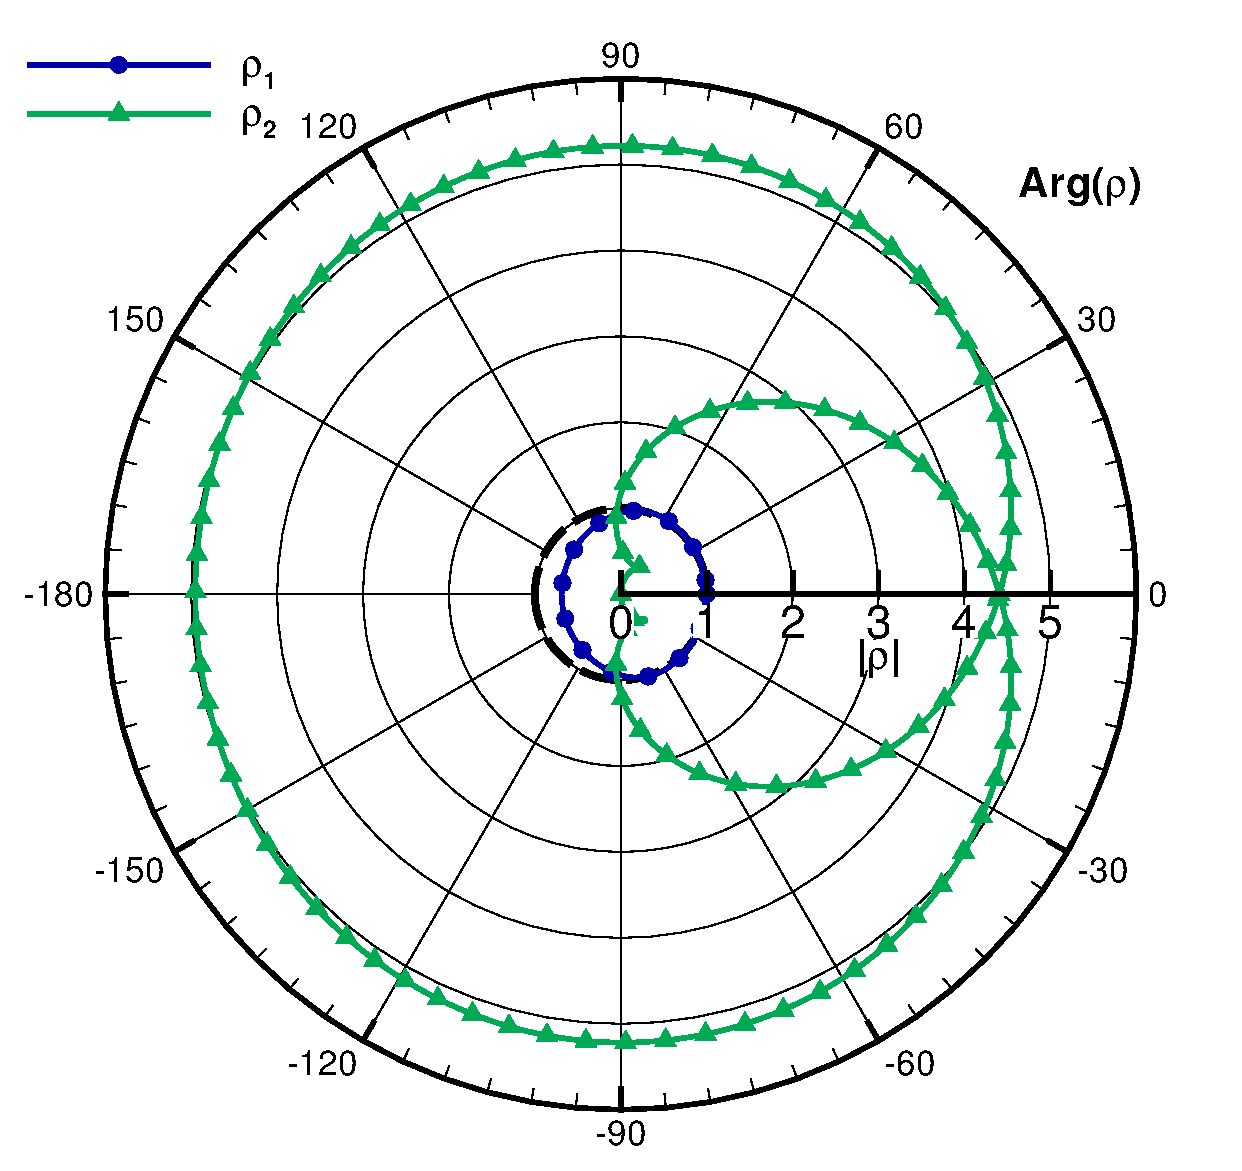
\includegraphics[width=0.74\textwidth]{fig/1D/pol62.pdf}
  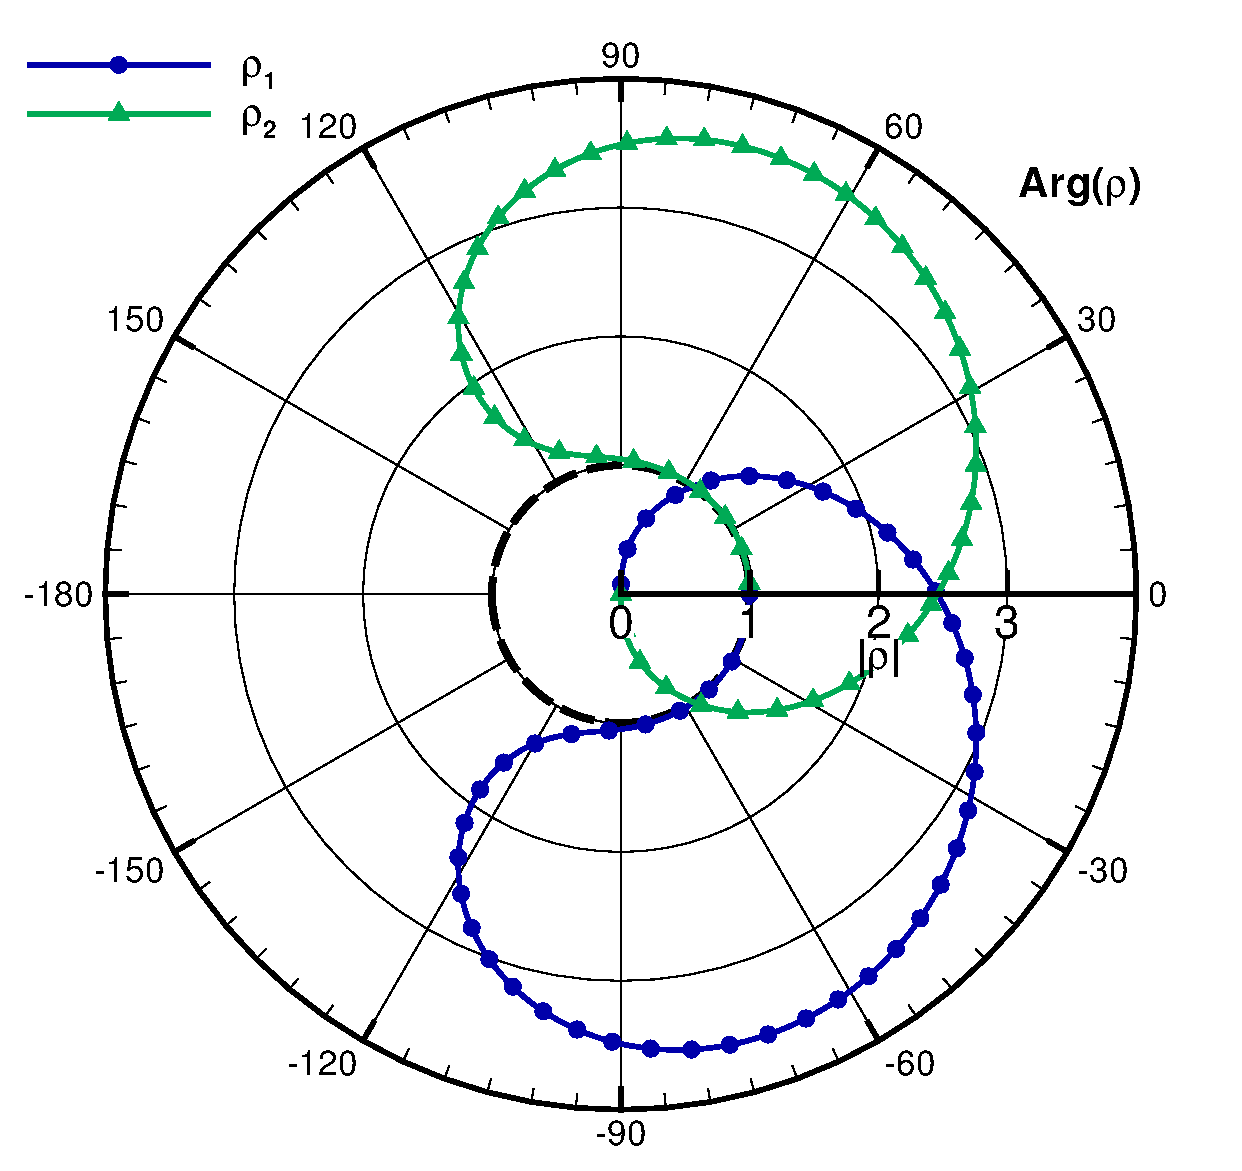
\includegraphics[width=0.74\textwidth]{fig/1D/pol80.pdf}
  \caption{$\rho_m(G)$在复平面的值。
    上:$k=3$,
    $r=2$,
    下:$k=4$,
    $r=0$。
    $k$是模板含有的单元数,
    $r$是 \cref{eq:stencils} 中定义的模板的偏移量,
    $\kappa h\in [0,2\pi]$,
    蓝色和绿色的线分别对应特征值$\rho_1(G)$和$\rho_2(G)$。
  }
  \label{fig:eigens-3}
\end{figure}

\begin{figure}[htbp]
  \centering
  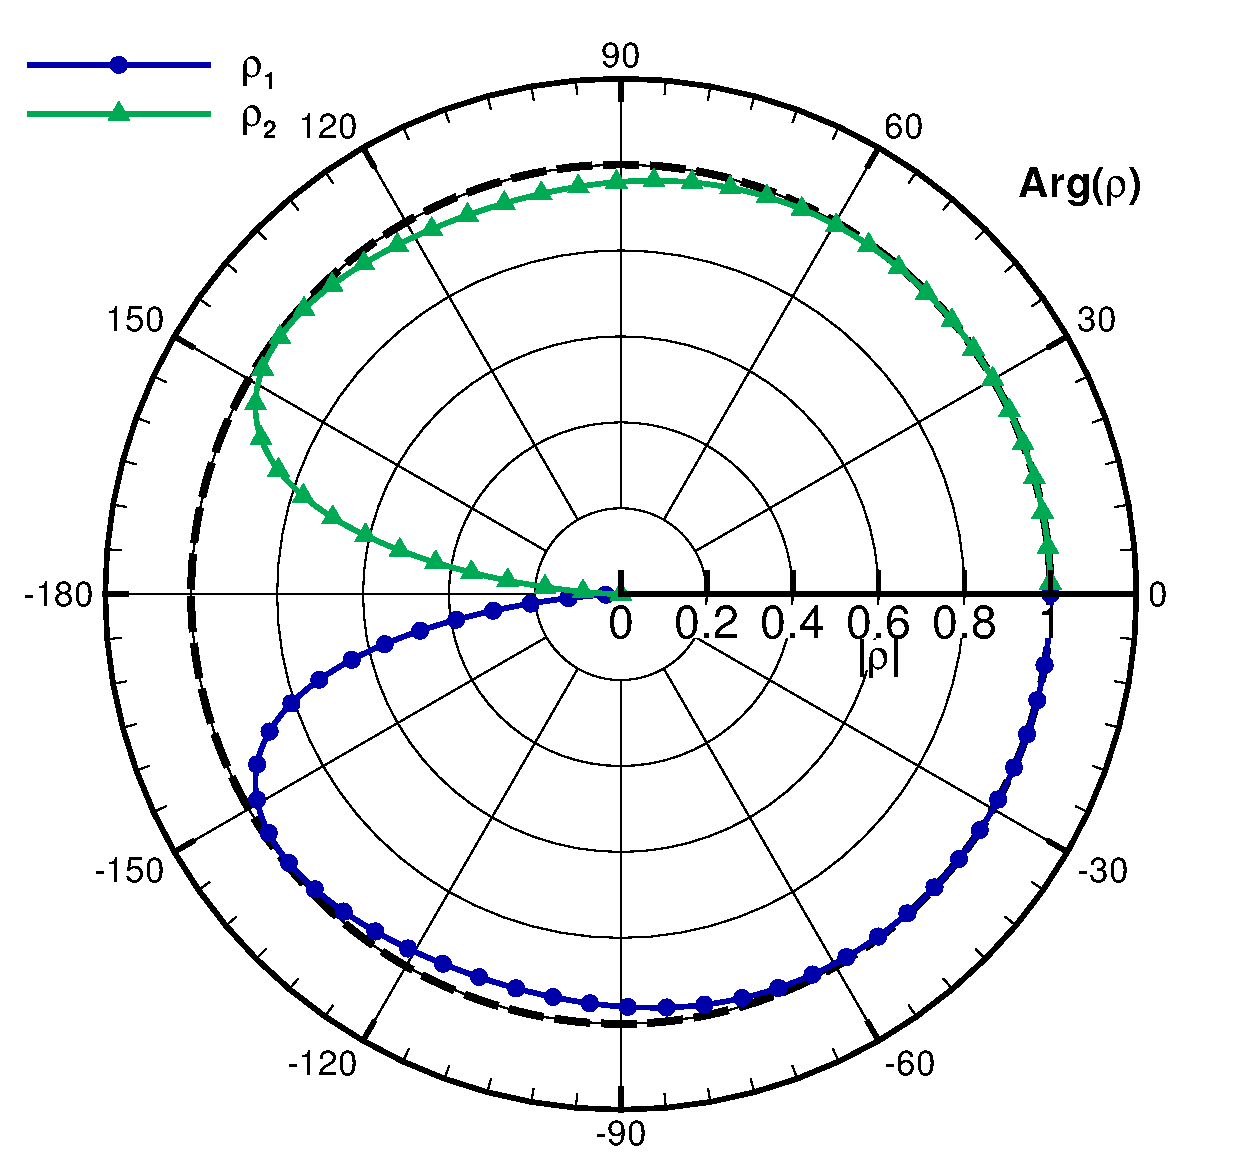
\includegraphics[width=0.74\textwidth]{fig/1D/pol81.pdf}
  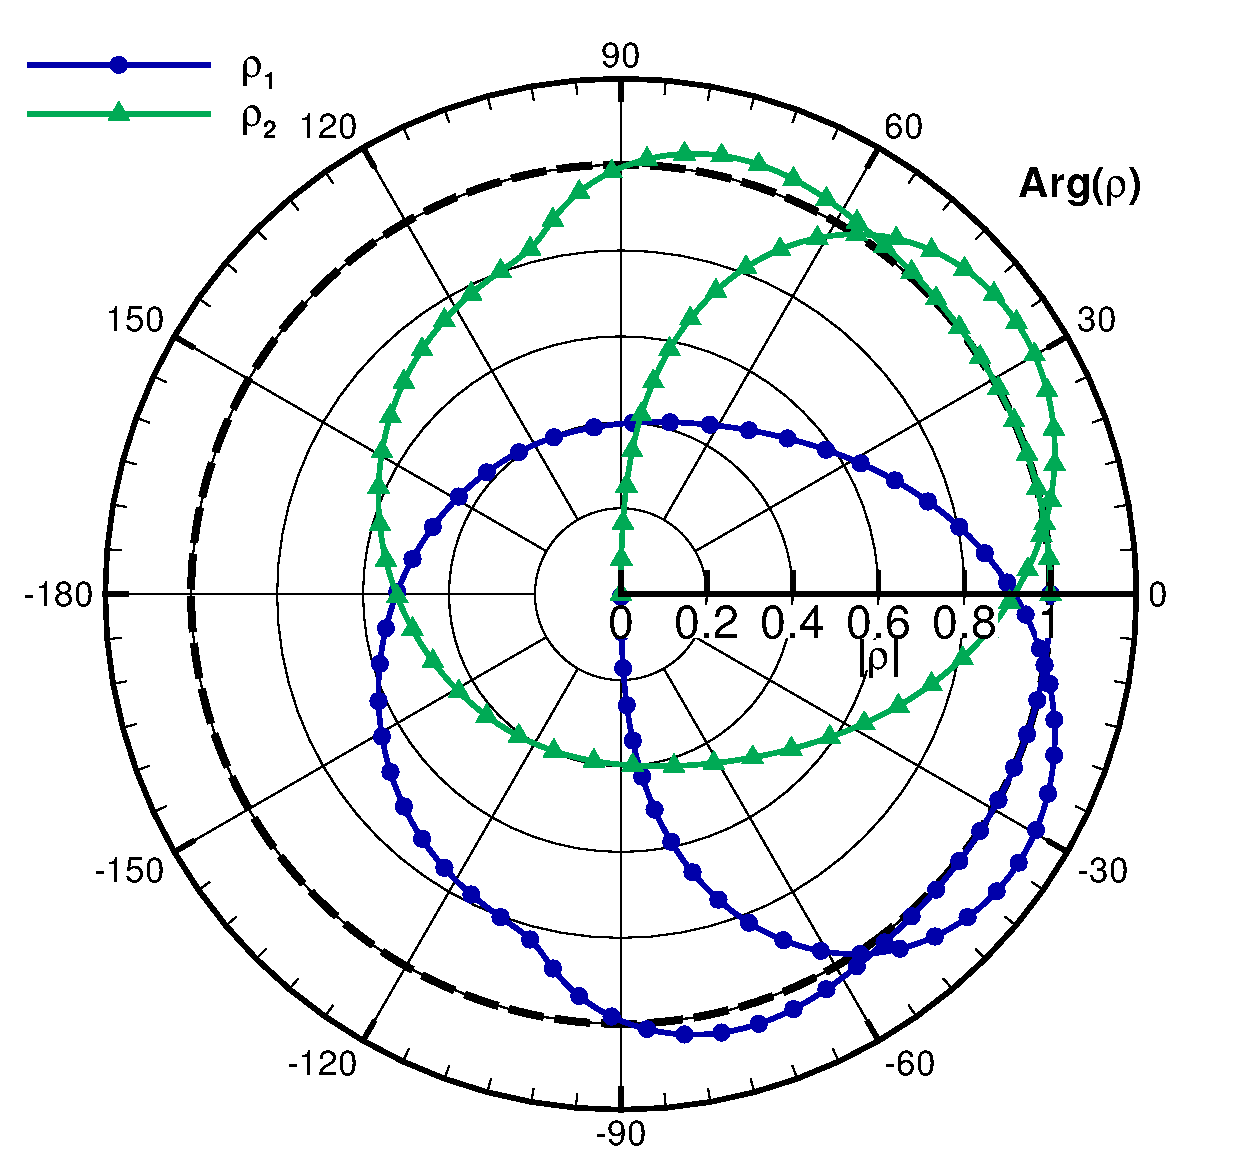
\includegraphics[width=0.74\textwidth]{fig/1D/pol82.pdf}
  \caption{$\rho_m(G)$在复平面的值。
    上:$k=4$,
    $r=1$,
    下:$k=4$,
    $r=2$。
    $k$是模板含有的单元数,
    $r$是 \cref{eq:stencils} 中定义的模板的偏移量,
    $\kappa h\in [0,2\pi]$,
    蓝色和绿色的线分别对应特征值$\rho_1(G)$和$\rho_2(G)$。
  }
  \label{fig:eigens-4}
\end{figure}

\begin{figure}[htbp]
  \centering
  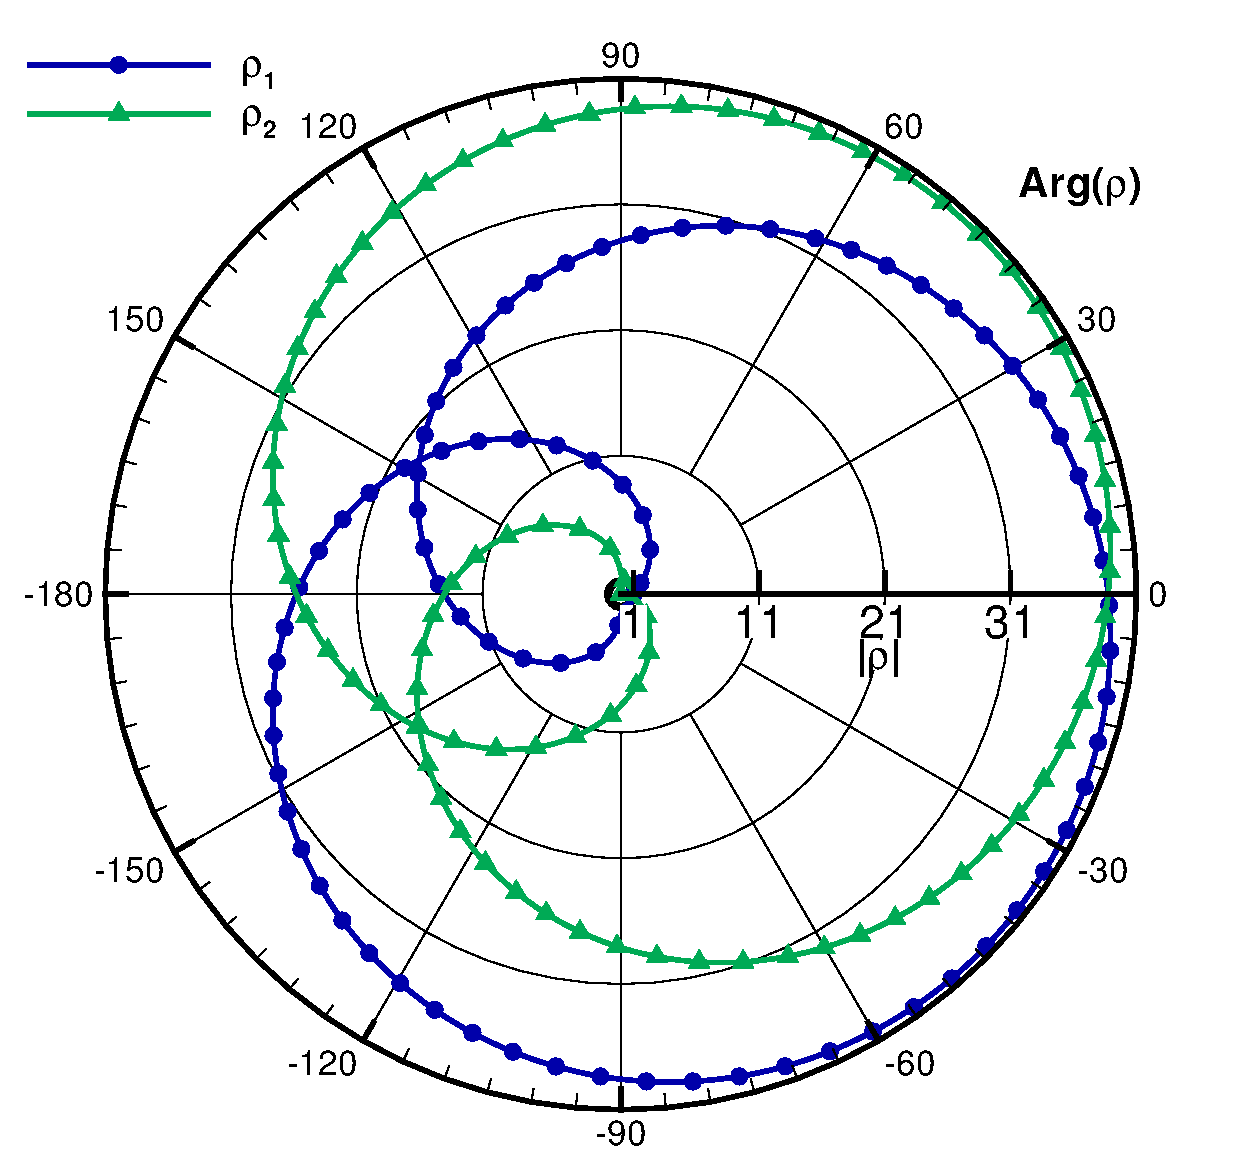
\includegraphics[width=0.74\textwidth]{fig/1D/pol83.pdf}
  \caption{$\rho_m(G)$在复平面的值。
    $k=4$,
    $r=3$。
    $k$是模板含有的单元数,
    $r$是 \cref{eq:stencils} 中定义的模板的偏移量,
    $\kappa h\in [0,2\pi]$,
    蓝色和绿色的线分别对应特征值$\rho_1(G)$和$\rho_2(G)$。
  }
  \label{fig:eigens-5}
\end{figure}

我们对重构多项式$p^r_i(x)$在$x=x_{i+\frac 12}$选取的模板有如下结论。

\begin{enumerate}
  \item 当$k=2$时,
        $S^2_0(i)= I_{i}\cup I_{i+1}$是一个好的模板,
        因为其特征值位于单位圆内,
        得到的数值格式是一个稳定的格式。
        不过$S^2_1(i)= I_{i-1}\cup I_{i}$不是。
        自然的,
        我们选择模板$S^2_0(i)$,
        得到一个稳定的两步四阶格式。
        这个重构是我们所期望构造的一维线性埃尔米特重构,
        得到的格式是我们所期望设计的一维两步四阶格式。
  \item 当$k=3$时,
        $S^3_1(i)$是一个好的模板,
        而其他两个表现的不好。
  \item 当$k=4$时,
        $S^4_1(i)$是一个好的模板,
        其他三个表现的都不好。
        同时,
        这个重构模板恰好与文\cite{zhao2019compact}中的八阶重构模板相同。
\end{enumerate}

自然的,
如果风向是反方向的,
即$\widetilde{C}<0$,
模板的选择也是相反的。
举个例子,
当$k=4$时,
我们会选择$S^4_2(i+1)=I_{i-1}\cup I_{i}\cup I_{i+1}\cup I_{i+2}$来构造多项式$p_{2,i+1}(x)$,
并进一步得到$x_{i+\frac 12}$处的值。

\begin{remark}
  这一数值得到的结果与“稳定性原则”一致:对于一个收敛的数值格式,
  其依赖域必须包含迎风的成分,
  而且尽可能接近相应的偏微分方程的依赖域。
\end{remark}

\begin{remark}
  当采用两步四阶时间推进框架求解方程组时,
  根据迎风原理,
  $u_{i+\frac{1}{2},-}$采用$\widetilde{C}>0$时以$I_i$为中心的模板;而$u_{i+\frac{1}{2},+}$采用$\widetilde{C}<0$时以$I_{i+1}$为中心的模板。
\end{remark}

\vspace{\baselineskip} % 节的总结
这一节中,
我们构造了在一维情形下的线性紧致埃尔米特重构,
并设计了相应的线性格式。
一共有三个稳定的格式,
根据它们的阶数不同,
分别记作HC-4、HC-6和HC-8格式。
其中的“HC”代表埃尔米特构造(Hermite Construction)。
其中的HC-4格式就是我们所期望设计的四阶的基于紧致埃尔米特重构的两步四阶格式的线性版本,
下面为了在间断附近避免数值振荡,
我们将构造非线性的重构,
并设计相应的基本无振荡格式。

\section{基本无振荡的紧致埃尔米特重构及其相应的两步四阶格式}

我们在\cref{sec:1D-linear-rec}中构造了线性紧致埃尔米特重构,
并设计了相应的线性格式,
它们在光滑区域可以保持高阶精度,
但是在间断附近会出现数值振荡。
为了设计格式能够在光滑区域保持高阶精度,
并同时有效防止间断附近出现数值振荡,
本节中我们在一维情形下,
构造两种基本无振荡的非线性重构,
即加权型和杂交选择型的紧致埃尔米特重构。
然后,
我们将设计相应的两步四阶格式。

\subsection{加权型紧致埃尔米特重构}
\label{sec:1D-WHC}

在文\cite{WENO-1996}中提出的非线性的WENO重构,
是一种有代表性的方法。
这引发了大量旨在优化其模板选择的后续研究,
包括CWENO\upcite{CWENO-origin,CWENO13579}和WENO-AO\upcite{WENOAO}格式,
这些先进的技术能够组合多个不同阶精度的重构。
还有一些旨在优化WENO重构中的非线性权构造的后续研究,
例如WENO-Z\upcite{WENO_Z}格式。
下面我们利用类似的技术,
推导加权型的紧致埃尔米特重构。

\subsubsection{加权型紧致埃尔米特重构的组成成分}

在\cref{sec:1D-linear-rec}中,
我们得到了二阶、四阶、六阶和八阶的线性埃尔米特重构。
值得注意的是,
二阶的重构与文\cite{Book-Matania}中广义黎曼问题格式使用的重构是一样的,
该格式在应对数值振荡方面表现出色。
为了达到相似的性能,
我们对 \cref{eq:1D-HC2} 中的$p_{i}(x)$应用与文\cite{Book-Matania}中相同的minmod限制器,
得到
\begin{align}
  \label{eq:1D-minmod-limiter}
   & \bar v^{lim}_{i} = \frac{1}{h}\mbox{minmod}(\alpha(\bar u_{i+1}-\bar u_{i}), h_x\bar v_{i}, \alpha(\bar u_{i}-\bar u_{i-1})), \\
   & p^{{s}}_{i}(x) = \bar u_{i}+ \bar v^{lim}_{i}(x-x_{i}),
\end{align}
其中,
参数$\alpha$在区间$[1,2)$内。
在本章的数值算例中,
我们将$\alpha$的值设为$1.9$。
符号“${{s}}$”被用来表示这个表达式是由二阶(second order)重构得出的。
在本节中,
我们仅关注多项式在$x_{i+\frac{1}{2}}$处的值,
即
\begin{equation}
  u_{i+\frac{1}{2},-}^{{s}}= p^{{s}}_{i}(x_{i+\frac{1}{2}}), \quad
  \left({\partial_{x}^{d}}u\right)_{i+\frac{1}{2},-}^{{s}}= {\partial_{x}^{d}}p_{i}^{{s}}(x_{i+\frac{1}{2}}), \quad d=1,2.
\end{equation}

另一方面,
四阶重构正好与两步四阶时间推进框架的精度匹配,
因此我们可以预期在光滑区域中达到四阶精度。
同样,
我们定义了符号
\begin{equation}
  u_{i+\frac{1}{2},-}^{{f}}= p^{{f}}_{i}(x_{i+\frac{1}{2}}), \quad
  \left({\partial_{x}^{d}}u\right)_{i+\frac{1}{2},-}^{{f}}= {\partial_{x}^{d}}p_{i}^{{f}}(x_{i+\frac{1}{2}}), \quad d=1,2,
\end{equation}
这些值是由四阶线性重构得到的,
其中“${{f}}$”表示由四阶(fourth order)重构得出的。

\subsubsection{加权型紧致埃尔米特重构的推导}

现在,
我们借鉴CWENO和WENO-AO格式中使用的技术来推导我们的加权型重构。
我们将从四阶线性重构得到的值$u_{i+\frac{1}{2},-}^{{f}}$重写为
\begin{equation}
  u_{i+\frac{1}{2},-}^{{f}}= \gamma_{{s}}u_{i+\frac{1}{2},-}^{{s}}+ \gamma_{{f}}\left(\frac{1}{\gamma_{{f}}}u_{i+\frac{1}{2},-}^{{f}}-\frac{\gamma_{{s}}}{\gamma_{{f}}}u_{i+\frac{1}{2},-}^{{s}}\right), \quad \gamma_{{s}}+ \gamma_{{f}}=1,
\end{equation}
其中,
$\gamma_{{s}}$和$\gamma_{{f}}$是线性权。
在实际数值算例中,
线性权$\gamma_{{s}}$和$\gamma_{{f}}$的值通常选择为0.1和0.9。
随后,
将线性权$\gamma_{{o}}$用非线性权$\omega_{{o}}$替代,
其中${{o}}={{s}}, {{f}}$代表精度阶数,
得到
\begin{equation}
  u_{i+\frac{1}{2},-}^{\text{WHC-4}}= \omega_{{s}}u_{i+\frac{1}{2},-}^{{s}}+ \omega_{{f}}\left(\frac{1}{\gamma_{{f}}}u_{i+\frac{1}{2},-}^{{f}}-\frac{\gamma_{{s}}}{\gamma_{{f}}}u_{i+\frac{1}{2},-}^{{s}}\right), \quad \omega_{{s}}+\omega_{{f}}=1,
\end{equation}
这里,
上标“WHC”代表加权埃尔米特构造(Weighted Hermite Construction),
相应的四阶重构被称为WHC-4重构。
这个表达式可以进一步简化为
\begin{equation}
  \label{eq:1D-WHC4}
  u_{i+\frac{1}{2},-}^{\text{WHC-4}}= \frac{\omega_{{f}}}{\gamma_{{f}}}u_{i+\frac{1}{2},-}^{{f}}+ \left(1-\frac{\omega_{{f}}}{\gamma_{{f}}}\right)u_{i+\frac{1}{2},-}^{{s}}.
\end{equation}

本章中的非线性权的定义方式参考文\cite{WENO_Z}中的WENO-Z格式。
这些非线性权的表达式为
\begin{equation}
  \label{eq:1D-nonlinearweight}
  \omega_{{o}}=\frac{\alpha_{{o}}}{\alpha_{{s}}+\alpha_{{f}}}, \quad
  \alpha_{{o}}=\gamma_{{o}}\left( 1+\left( \frac{\theta}{\beta_{{o}}+\varepsilon}\right)^q \right) , \quad {{o}}={{s}}, {{f}},
\end{equation}
其中,
变量$\theta$是$\beta_{{s}}$和$\beta_{{f}}$的差的绝对值,
即$\theta = |\beta_{{s}}-\beta_{{f}}|$。
小量$\varepsilon$的表达式是$\widehat{C}h^3$,
其中$\widehat{C}$在我们的数值算例中设为100。
幂指数$q$设为2。

光滑因子$\beta_{{s}}$和$\beta_{{f}}$采取类似于文\cite{WENO-1996}中使用的定义,
即一维的情形下为
\begin{equation}
  \beta_{{o}}= \sum_{d=1}^3 \int_{I_{i}}h^{2\ell-1}\left({\partial_{x}^{d}}p^{{o}}_{i}(x)\right)^2 dx, \quad {{o}}={{s}},{{f}},
\end{equation}
在均匀网格的情况下,
具体的表达式可以写为
\begin{align}
   & \beta_{{s}}=
  (h \bar v_{i})^2,                                                                                                                                            \\
   & \begin{aligned}
       \beta_{{f}}=
        & \frac{13}{3}\left(-3 \bar u_{i}+ 3 \bar u_{i+1}- 2 \bar v_{i}-\bar v_{i+1}\right)^2 +
       \frac{1}{16}\left(-2 \bar u_{i}+ 2 \bar u_{i+1}+ 3 \bar v_{i}-\bar v_{i+1}\right)^2                                                                    \\
        & + \frac{1}{8}\left(-2 \bar u_{i}+ 2 \bar u_{i+1}+ 3 \bar v_{i}-\bar v_{i+1}\right)\left(2 \bar u_{i}- 2 \bar u_{i+1}+\bar v_{i}+\bar v_{i+1}\right) \\
        & +\frac{3129}{80} \left(2 \bar u_{i}- 2 \bar u_{i+1}+\bar v_{i}+\bar v_{i+1}\right)^2.
     \end{aligned}
\end{align}

我们继续使用与 \cref{eq:1D-nonlinearweight} 中相同的非线性权,
可以在$x_{i+\frac{1}{2}}$处得到一阶和二阶空间导数,
即
\begin{equation}
  \left({\partial_{x}^{d}}u\right)_{i+\frac{1}{2},-}^{\text{WHC-4}}= \frac{\omega_{{f}}}{\gamma_{{f}}}\left({\partial_{x}^{d}}u\right)_{i+\frac{1}{2},-}^{{f}}+ \left(1-\frac{\omega_{{f}}}{\gamma_{{f}}}\right)\left({\partial_{x}^{d}}u\right)_{i+\frac{1}{2},-}^{{s}}, \quad d=1,2.
\end{equation}
在计算导数的重构时,
几乎没有额外的计算代价,
因为不必重新计算非线性权。

\subsubsection{加权型紧致埃尔米特重构的性质}

我们现在已经得到了四阶加权型埃尔米特重构。
接下来,
我们将验证这种重构的性质。
不失一般性,
我们采用均匀网格。
此时可以得到光滑因子在光滑区域的$x_{i}$处的泰勒展开:
\begin{equation}
  \label{eq:1D-Taylor}
  \begin{aligned}
     & \beta_{{s}}=\xi_1 h^2+\frac{1}{12}\xi_3 h^4+{\mathcal{O}}(h^6), \quad
    \beta_{{f}}=\xi_1 h^2 +\frac{1}{12}(\xi_2+\xi_3) h^4 +{\mathcal{O}}(h^6),        \\
     & \theta = |\beta_{{s}}-\beta_{{f}}|=\frac{1}{12}\xi_2 h^4+{\mathcal{O}}(h^6),
  \end{aligned}
\end{equation}
其中$\xi_1$、$\xi_2$和$\xi_3$的定义如下
\begin{equation}
  \xi_1=\left({\partial_{x}}u\right)^2, \quad
  \xi_2=13\left({\partial_{x}^2}u\right)^2, \quad
  \xi_3={\partial_{x}}u \cdot {\partial_{x}^3} u.
\end{equation}

随后,
我们根据非线性权的定义 \cref{eq:1D-nonlinearweight} 可以得到非线性权在光滑区域内满足以下关系
\begin{equation}
  \omega_{{o}}= \gamma_{{o}}+ {\mathcal{O}}(h^2) , \quad {{o}}={{s}}, {{f}}.
\end{equation}
因此,
我们得到$u_{i+\frac{1}{2},-}^{\text{WHC-4}}$是对精确值$u(x_{i+\frac{1}{2}})$的四阶精确近似,
如下式所示
\begin{equation}
  u_{i+\frac{1}{2},-}^{\text{WHC-4}}= u_{i+\frac{1}{2},-}^{{f}}+ \frac{\omega_{{f}}- \gamma_{{f}}}{\gamma_{{f}}}\left(u_{i+\frac{1}{2},-}^{{f}}-u_{i+\frac{1}{2},-}^{{s}}\right) = u_{i+\frac{1}{2},-}^{{f}}+ {\mathcal{O}}(h^4)= u(x_{i+\frac{1}{2}})+{\mathcal{O}}(h^4).
\end{equation}

在间断附近,
我们有
\begin{equation}
  \omega_{{s}}= 1-{\mathcal{O}}(h^4), \quad \omega_{{f}}= {\mathcal{O}}(h^4),
\end{equation}
也就是$\omega_{{s}}$接近于$1$,
使得二阶的重构起主要作用,
从而可有效防止振荡。

综上所述,
我们从理论上论证了该重构可以在光滑区域保持高阶精度,
同时可以有效防止间断附近的出现数值振荡。

\subsubsection{八阶加权型紧致埃尔米特重构}

由于六阶线性埃尔米特重构对应的数值格式HC-6格式在求解非线性方程组(如欧拉方程组)时,
遇到了数值不稳定的问题,
如\cref{ta:1D-ex2-HC6} 所示,
我们不再将之发展到非线性重构。
这里将八阶线性埃尔米特重构发展到加权型紧致埃尔米特重构。
此时,
需要对现有的加权型紧致埃尔米特重构进行微小的修改:
\begin{enumerate}
  \item 用从八阶重构导出的多项式$p^{{e}}(x,y)$替换$p^{{f}}(x,y)$。
  \item 重新计算相应的光滑因子。
  \item 调整 \cref{eq:1D-nonlinearweight} 中的幂指数$q$为3。
\end{enumerate}

\vspace{0.5\baselineskip} % 小节的总结
本小节中,
我们在一维情形下,
构造了四阶和八阶的加权型紧致埃尔米特重构。
这些重构分别被称为WHC-4和WHC-8重构。

\subsection{杂交选择型紧致埃尔米特重构}

在加权型紧致埃尔米特重构中,
计算了两个候选模板的重构值,
并选择它们的凸组合作为最终的重构值。
然而,
在光滑区域,
只有高阶重构的计算有价值,
而在间断附近,
只有低阶重构发挥了避免振荡的效果。
因此,
基于对加权型重构的分析,
我们得到了杂交选择策略,
这可能是一种更有效的重构方法。
这种策略最初是在文\cite{hybrid-first}中提出的,
已经被广泛应用于许多研究中\upcite{hybrid-2015}。

\subsubsection{杂交选择型紧致埃尔米特重构的推导}

我们先回顾 \cref{eq:1D-WHC4}:
\begin{equation*}
  u_{i+\frac{1}{2},-}^{\text{WHC-4}}= \frac{\omega_{{f}}}{\gamma_{{f}}}u_{i+\frac{1}{2},-}^{{f}}+ \left(1 - \frac{\omega_{{f}}}{\gamma_{{f}}}\right) {u}_{i+\frac{1}{2},-}^{{s}}.
\end{equation*}
我们观察到,
第一项的系数${\omega_{{f}}}/{\gamma_{{f}}}$在光滑区域趋近于$1$,
而在间断附近,
这个系数趋近于$0$。
因此,
我们可以对 \cref{eq:1D-WHC4} 应用一个截断函数,
得到我们的杂交选择型重构
\begin{equation}
  \label{eq:1D-HHC4-perpare}
  u_{i+\frac{1}{2},-}^{\text{HHC-4}}= \delta\left(\frac{\omega_{{f}}}{\gamma_{{f}}}\right) u_{i+\frac{1}{2},-}^{{f}}+ \left(1-\delta\left(\frac{\omega_{{f}}}{\gamma_{{f}}}\right) \right) {u}_{i+\frac{1}{2},-}^{{s}}.
\end{equation}
这里,
上标“HHC”代表杂交埃尔米特构造(Hybrid Hermite Construction),
截断函数$\delta$的定义是
\begin{equation}
  \label{eq:1D-truncation-function}
  \delta(\xi) =
  \begin{cases}
    1, & \xi > {C}/{\gamma_{{f}}},   \\
    0, & \xi \le{C}/{\gamma_{{f}}},
  \end{cases}
\end{equation}
其中,
$C$是一个位于区间$(0,\gamma_{{f}})$内的阈值。
然后 \cref{eq:1D-HHC4-perpare} 就等价于
\begin{equation}
  \label{eq:1D-HHC-4}
  \begin{aligned}
    u_{i+\frac{1}{2},-}^{\text{HHC-4}}=
    \begin{cases}
      u_{i+\frac{1}{2},-}^{{f}}, & \omega_{{f}}> C ,   \\
      u_{i+\frac{1}{2},-}^{{s}}, & \omega_{{f}}\le C.
    \end{cases}
  \end{aligned}
\end{equation}
由于非线性权$\omega_{{f}}$的计算较为复杂,
我们希望探寻$\omega_{{f}}> C$是否可以被一个计算更便宜的不等式替代。
将 \cref{eq:1D-nonlinearweight} 代入$\omega_{{f}}> C$,
我们得到
\begin{equation}
  \label{eq:1D-inequation1}
  1+\left(\frac{\beta_{{s}}- \beta_{{f}}}{\beta_{{f}}+ \varepsilon}\right)^2 > \frac{C\gamma_{{s}}}{(1-C)\gamma_{{f}}}\left(1+\left(\frac{\beta_{{s}}- \beta_{{f}}}{\beta_{{s}}+ \varepsilon}\right)^2\right).
\end{equation}
设$\vartheta = (\beta_{{f}}+\varepsilon)/(\beta_{{s}}+\varepsilon)$和$E=(1-C)/C \cdot \gamma_{{f}}/\gamma_{{s}}$。
那么有$\vartheta>0$和$E>1$。
我们注意到对于固定的$C$,
$E$实际上是一个常数,
因为$\gamma_{{s}}$和$\gamma_{{f}}$是固定的线性权。
由于下式成立
\begin{equation}
  \frac{\beta_{{s}}- \beta_{{f}}}{\beta_{{f}}+\varepsilon}=\frac 1\vartheta-1,
\end{equation}
我们将 \cref{eq:1D-inequation1} 重写为
\begin{equation}
  \label{eq:1D-inequation2}
  g(E,\vartheta) \coloneqq (E-1)\vartheta^2+(1-\vartheta)^2(E-\vartheta^2)>0.
\end{equation}
记
\begin{equation}
  s(\vartheta)=\dfrac{\vartheta^2((1-\vartheta)^2+1)}{((1-\vartheta)^2+\vartheta^2)},
\end{equation}
则有$g(s(\vartheta), \vartheta)=0$,
同时我们注意到$s(\vartheta)$作为$\vartheta>0$的函数是单调递增的,
这意味着$E>s(\vartheta)$成立等价于 \cref{eq:1D-inequation2} 成立。
我们设$\bar \vartheta= s^{-1}(E)$,
这样 \cref{eq:1D-inequation1} 成立就等价于
\begin{equation}
  \label{eq:1D-inequation3}
  0<\vartheta<\bar\vartheta.
\end{equation}
因此,
我们用 \cref{eq:1D-inequation3} 替换 \cref{eq:1D-HHC-4} 中的$\omega_{{f}}>C$,
得到
\begin{equation}
  \label{eq:1D-HHC4}
  \begin{aligned}
    u_{i+\frac{1}{2},-}^{\text{HHC-4}}=
    \begin{cases}
      u_{i+\frac{1}{2},-}^{{f}}, & \beta_{{f}}+\varepsilon < \bar{\vartheta}(\beta_{{s}}+\varepsilon),   \\
      u_{i+\frac{1}{2},-}^{{s}}, & \beta_{{f}}+\varepsilon \ge\bar{\vartheta}(\beta_{{s}}+\varepsilon).
    \end{cases}
  \end{aligned}
\end{equation}
这是我们最终的HHC-4重构。
与WHC-4重构相比,
它避免了计算非线性权$\omega_{{s}}$和$\omega_{{f}}$。
\begin{remark}
  最初在 \cref{eq:1D-HHC-4} 中,
  我们需要给定$C$。
  然后由于$\bar\vartheta$和$C$之间有直接的一一映射关系,
  现在我们只需在 \cref{eq:1D-HHC4} 中给定阈值$\bar\vartheta$。
\end{remark}

\subsubsection{杂交选择型紧致埃尔米特重构中参数$\bar\vartheta$的选择}

我们注意到 \cref{eq:1D-HHC4} 中的不等式可以理解为$\vartheta$和阈值$\bar\vartheta$之间的比较。
经过仔细分析,
我们发现在光滑区域,
$\vartheta$接近于$1$,
满足
\begin{equation}
  \label{eq:1D-vartheta-in-smooth}
  \vartheta = \frac{\beta_{{f}}+ \varepsilon}{\beta_{{s}}+ \varepsilon}
  = 1 + \frac{\beta_{{f}}- \beta_{{s}}}{\beta_{{s}}+ \varepsilon}= 1 + {\mathcal{O}}(h),
\end{equation}
然而,
在有物理振荡的光滑区域,
例如数值算例中的Titarev-Toro问题,
\cref{eq:1D-vartheta-in-smooth} 中$h$的系数可能非常大,
以至于$\vartheta$的值远离$1$。
在间断附近,
它是一个相对较大的数,
满足
\begin{equation}
  \vartheta = \frac{\beta_{{f}}+ \varepsilon}{\beta_{{s}}+ \varepsilon}= {\mathcal{O}}(h^{-2}),
\end{equation}
然而,
当间断不强时,
$\vartheta$的值并不是很大。
换句话说,
一些弱间断附近的$\vartheta$值,
可能会接近有物理振荡的光滑区域中的$\vartheta$值。
因此很难使用$\vartheta$清楚地区分那些有物理振荡的光滑区域和接近弱间断的区域。
$\vartheta$和$\bar\vartheta$的关系示意图展示在\cref{fig:1D-vartheta} 中,
展示了$\vartheta$在光滑区域、混合区域和间断附近区域的值的关系。
混合区域指一些高频振荡的光滑区域和接近弱间断的区域是混合在一起的。
因此,
我们必须适当地选择$\bar\vartheta$,
一维情形下建议取$50$。

回顾 \cref{eq:1D-HHC4},
可以观察到,
$\bar\vartheta$的取值越大,
高阶多项式被使用的比例就越大。
我们可以据此调整$\bar\vartheta$以获得满意的解。

\begin{figure}[htbp]
  \centering
  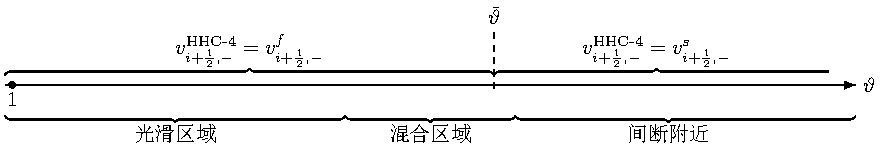
\includegraphics{fig/tikz/vartheta-1D.pdf}
  \caption{$\vartheta$和$\bar\vartheta$的关系示意图。
  }
  \label{fig:1D-vartheta}
\end{figure}

\subsubsection{八阶杂交选择型紧致埃尔米特重构}

我们在这里可以将八阶线性重构发展到杂交选择型紧致埃尔米特重构,
需要对现有的杂交选择型紧致埃尔米特重构进行微小的修改:
\begin{enumerate}
  \item 用从八阶重构导出的多项式$p^{{e}}(x,y)$替换$p^{{f}}(x,y)$。
  \item 重新计算相应的光滑因子。
  \item 重新选择新的阈值$\bar\vartheta$。
\end{enumerate}
此时,
推荐的阈值$\bar\vartheta$与四阶重构的情况不同,
我们建议取$500000$。

\vspace{0.5\baselineskip} % 小节的总结
本小节中,
我们在一维情形下,
构造了四阶和八阶的杂交选择型紧致埃尔米特重构。
这些重构分别被称为HHC-4和HHC-8重构。

\subsection{基于紧致埃尔米特重构的基本无振荡的两步四阶格式}

下面我们基于紧致埃尔米特重构,
设计一维基本无振荡的紧致两步四阶格式。
我们使用在\cref{sec:1D-S2O4}中提出的改进的两步四阶时间推进框架,
其中的重构$\mathcal{R}$采用已经得到的两个四阶的紧致埃尔米特重构WHC-4和HHC-4重构,
LW型解法器$\mathcal{G}$采用\cref{sec:1D-solver-sec3}中介绍的Godunov解法器和广义黎曼问题解法器。
然后,
我们得到了相应的数值格式——WHC-4和HHC-4格式。
类似的,
我们也可以得到WHC-8和HHC-8格式。

关于WHC-4和HHC-4格式,
我们有以下论述。
\begin{enumerate}
  \item HHC-4重构通过直接比较光滑因子来选取合适的模板,
        使其比WHC-4重构更高效。
  \item 在间断附近,
        HHC-4重构完全采用HC-2重构,
        这在应对间断方面表现出了强大的数值性能。
  \item 在光滑区域,
        HHC-4重构只采用HC-4重构,
        这使得数值格式具有更小的误差。
  \item 另一方面,
        HHC-4重构对单元平均值和导数平均值的依赖不连续,
        在$\vartheta$接近$\bar\vartheta$的区域,
        由于舍入误差的小扰动,
        选择可能会有所不同,
        并导致重构结果的突变。
\end{enumerate}

\subsection{数值格式的紧致性}

在本小节,
我们将讨论一维数值格式的紧致性。
对于特定的数值格式,
如果它在一个单元依赖的前一个时间层上的单元越少,
那么该格式就越紧致。
以我们的WHC-4格式为例。
重构值${\bm{u}}_{i+\frac{1}{2},\pm}^{n}$、$({\partial_{x}}{\bm{u}})_{i+\frac{1}{2},\pm}^{n}$和$({\partial_{x}^2}{\bm{u}})_{i+\frac{1}{2},\pm}^{n}$,
在单元边界$x_{i+\frac{1}{2}}$的两侧,
如\cref{subfig:flux} 所示,
依赖于时间层$t=t^n$的$I_i$和$I_{i+1}$两个单元。
因此,
这个单元边界处的数值通量$\hat{\bm{f}}_{i+\frac{1}{2}}^*$和点值$\hat{\bm{u}}_{i+\frac{1}{2}}^{n+\frac{1}{2}}$依赖于这两个单元。
类似的,
单元$I_{i}$左侧边界上的数值通量和单元边界值依赖于$I_i$和$I_{i-1}$两个单元。
因此,
时间层$t=t^{n+\frac{1}{2}}$的平均值$\bar{\bm{u}}_{i}^{n+\frac{1}{2}}$和$\bar{\bm{v}}_{i}^{n+\frac{1}{2}}$依赖于时间层$t=t^n$的三个单元。
然后,
时间层$t=t^{n+1}$的平均值就依赖于时间层$t=t^n$的5个单元,
如\cref{subfig:1D-compact-HC4} 所示。
我们的HHC-4格式也是一样的。

作为对比,
文\cite{du2018hermite}中的S2O4-HWENO5格式,
它在时间层$t=t^{n+1}$的平均值依赖于时间层$t=t^n$的9个单元,
如\cref{subfig:flux2,subfig:1D-compact-HWENO5} 所示。
所以,
我们新设计的格式是一个更加紧致的格式。

\begin{figure}[htbp]
  \centering
  \subfigure[WHC-4和HHC-4格式的数值通量的依赖区域]{
    \label{subfig:flux}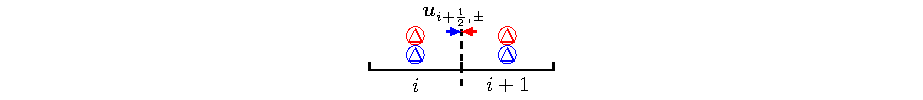
\includegraphics{fig/tikz/compact-1D-flux.pdf}
  } \\
  \subfigure[WHC-4和HHC-4格式的依赖区域]{
    \label{subfig:1D-compact-HC4}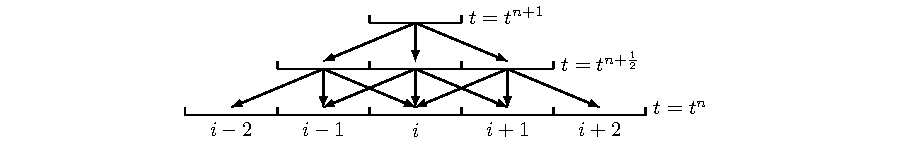
\includegraphics{fig/tikz/compact-1D-HC4.pdf}
  } \\
  \subfigure[文献\cite{du2018hermite}中的S2O4-HWENO5格式的数值通量的依赖区域]{
    \label{subfig:flux2}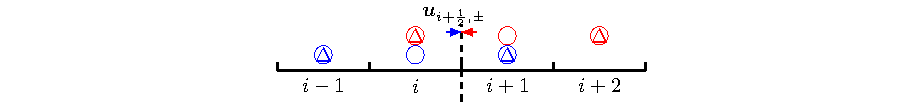
\includegraphics{fig/tikz/compact-1D-flux2.pdf}
  } \\
  \subfigure[文献\cite{du2018hermite}中的S2O4-HWENO5格式的依赖区域]{
    \label{subfig:1D-compact-HWENO5}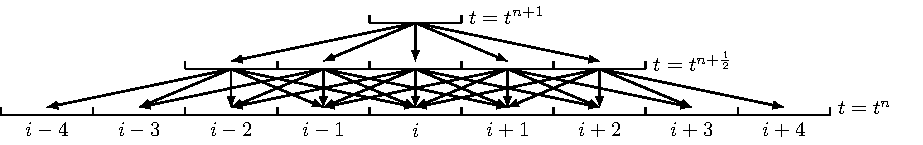
\includegraphics{fig/tikz/compact-1D-HWENO5.pdf}
  }
  \caption{这是依赖区域的示意图。
    标记${\bigcirc}$代表单元平均值,
    而标记${\Delta}$代表导数平均值。
    蓝色代表左侧重构值的依赖范围,
    而红色代表右侧重构值的依赖范围,
    两者的并集就是数值通量$\hat f^*_{i+\frac{1}{2}}$和单元边界值$\hat{\bm{u}}_{i+\frac{1}{2}}^{n+\frac{1}{2}}$的依赖区域。
  }
  \label{fig:1D-compactness}
\end{figure}

\vspace{\baselineskip} % 节的总结
本节中,
我们在一维情形下,
构造了两种基本无振荡的非线性重构,
即加权型和杂交选择型的紧致埃尔米特重构,
并设计了相应的基本无振荡的两步四阶格式。
一共四个格式,
分别记作WHC-4、WHC-8、HHC-4和HHC-8格式。
其中的WHC-4和HHC-4格式就是我们所期望设计的一维四阶的基于紧致埃尔米特重构的基本无振荡的两步四阶数值格式。

\section{数值实验}
\label{sec:1D-examples}

我们在一维情形下,
一共得到了三种线性紧致的两步四阶格式以及四种基本无振荡的紧致两步四阶格式——HC-4、HC-6、HC-8、WHC-4、WHC-8、HHC-4和HHC-8格式。
在这一节,
我们将用一些数值算例来测试它们的性能,
其中要重点测试我们设计的四阶精度格式HC-4、WHC-4和HHC-4格式。
对于所有的算例,
CFL数取$0.6$,
除了在\cref{ex:large-ratio} 中取$0.2$。
$\bar\vartheta$的值按照建议在所有的算例中取$50$,
除了在\cref{ex:toro} 中取$500$。
对于空间八阶的HHC-8格式,
阈值$\bar\vartheta$设定为$500000$。

在本节中,
我们提供了一些双曲守恒律 \cref{eq:1D-law} 的数值算例来展示我们的数值格式的性能。
双曲守恒律选取了两种,
分别是线性对流方程
\begin{equation}
  \label{eq:1D-linear}
  {\partial_{t}}u + {\partial_{x}}u = 0,
\end{equation}
和欧拉方程组
\begin{equation}
  \label{eq:1D-Euler}
  {\partial_{t}}{\bm{u}} + {\partial_{x}}{\bm{f}}({\bm{u}}) = 0, \quad
  {\bm{u}} =(\rho, \rho u, \rho E)^\top, \quad
  {\bm{f}}({\bm{u}}) =(\rho u,\rho u^2+p, u(\rho E+p))^\top,
\end{equation}
其中$\rho$、$u$和$p$分别是密度、速度和压力,
$E=u^2/2+e$是总能量,
$e$是内能,
对于多方气体有$e=p/((\gamma-1)\rho)$,
其中$\gamma$是多方指数,
如无特别说明取$1.4$。

\subsection{空间四阶精度的两步四阶格式}

\begin{example}[一维线性对流方程的精度测试]
  \label{ex:1D-acc1}
  这个算例选择线性对流方程 \cref{eq:1D-linear} 作为模型,
  初值为
  \begin{equation}
    u(x, 0) = 1 + 0.2\sin(\pi x).
  \end{equation}
  计算区域是$[-1,1]$,
  采取周期边界条件。
  这个问题的精确解是$u(x,t) = u(x-t,0)$。
\end{example}

对应于时间$t^{tem}=1$,
采用HC-4格式、WHC-4和HHC-4格式计算得到的变量$u$的单元平均值的误差见\cref{ta:1D-ex1-HC4,ta:1D-ex1-WHC4,ta:1D-ex1-HHC4},
其中的“Nstep”代表时间推进的次数。
所有的格式在光滑区域都达到了预期的精度阶数。

\def\titleintable{CFL&$h$&Nstep&$L^1$-error&$L^1$-order&$L^\infty$-error&$L^\infty$-order\\}
% \begin{table}[htbp]
% 	\caption{HC-4格式在例 \ref{ex:1D-acc1} 中$u$的$L^1$和$L^\infty$误差和误差阶。展示的是$t^{tem} = 1$时刻的结果。}
% 	\label{ta:1D-ex1-HC4}
% 	\centering
% 	\begin{tabular}{ccccccc}
% 		\toprule
% 		\titleintable
% 		\midrule
% 		0.6 & 2/40   & 34   & 1.39581e-06 &              & 2.19020e-06 &              \\
% 		0.6 & 2/80   & 67   & 8.73170e-08 & \hl{3.99869} & 1.37118e-07 & \hl{3.99757} \\
% 		0.6 & 2/160  & 134  & 5.45979e-09 & \hl{3.99935} & 8.57559e-09 & \hl{3.99904} \\
% 		0.6 & 2/320  & 267  & 3.41097e-10 & \hl{4.00059} & 5.35806e-10 & \hl{4.00045} \\
% 		0.6 & 2/640  & 534  & 2.12972e-11 & \hl{4.00144} & 3.35383e-11 & \hl{3.99783} \\
% 		0.6 & 2/1280 & 1067 & 1.33043e-12 & \hl{4.00071} & 2.39120e-12 & \hl{3.81000} \\
% 		\bottomrule
% 	\end{tabular}
% \end{table}

\begin{table}[htbp]
	\caption{WHC-4格式在例 \ref{ex:1D-acc1} 中$u$的$L^1$和$L^\infty$误差和误差阶。展示的是$t^{tem} = 1$时刻的结果。}
	\label{ta:1D-ex1-WHC4}
	\centering
	\begin{tabular}{ccccccc}
		\toprule
		\titleintable
		\midrule
		0.6 & 2/40   & 34   & 1.39581e-06 &              & 2.19020e-06 &              \\
		0.6 & 2/80   & 67   & 8.73170e-08 & \hl{3.99869} & 1.37118e-07 & \hl{3.99757} \\
		0.6 & 2/160  & 134  & 5.45979e-09 & \hl{3.99935} & 8.57559e-09 & \hl{3.99904} \\
		0.6 & 2/320  & 267  & 3.41097e-10 & \hl{4.00059} & 5.35806e-10 & \hl{4.00045} \\
		0.6 & 2/640  & 534  & 2.12974e-11 & \hl{4.00143} & 3.35378e-11 & \hl{3.99785} \\
		0.6 & 2/1280 & 1067 & 1.33042e-12 & \hl{4.00072} & 2.38898e-12 & \hl{3.81132} \\
		\bottomrule
	\end{tabular}
\end{table}

\begin{table}[htbp]
	\caption{HHC-4格式在例 \ref{ex:1D-acc1} 中$u$的$L^1$和$L^\infty$误差和误差阶。展示的是$t^{tem} = 1$时刻的结果。}
	\label{ta:1D-ex1-HHC4}
	\centering
	\begin{tabular}{ccccccc}
		\toprule
		\titleintable
		\midrule
		0.6 & 2/40   & 34   & 1.39581e-06 &              & 2.19020e-06 &              \\
		0.6 & 2/80   & 67   & 8.73170e-08 & \hl{3.99869} & 1.37118e-07 & \hl{3.99757} \\
		0.6 & 2/160  & 134  & 5.45979e-09 & \hl{3.99935} & 8.57559e-09 & \hl{3.99904} \\
		0.6 & 2/320  & 267  & 3.41097e-10 & \hl{4.00059} & 5.35806e-10 & \hl{4.00045} \\
		0.6 & 2/640  & 534  & 2.12972e-11 & \hl{4.00144} & 3.35383e-11 & \hl{3.99783} \\
		0.6 & 2/1280 & 1067 & 1.33043e-12 & \hl{4.00071} & 2.39120e-12 & \hl{3.81000} \\
		\bottomrule
	\end{tabular}
\end{table}
\undef\titleintable

\begin{example}[一维欧拉方程组的线性退化的精度测试]
  \label{ex:1D-acc2}
  这个算例选择欧拉方程组 \cref{eq:1D-Euler} 作为模型,
  其中多方指数$\gamma$取$1.4$,
  初值为
  \begin{equation}
    \rho(x, 0) = 1 + 0.2\sin(\pi x), \quad u(x,0)=1, \quad p(x,0)=1.
  \end{equation}
  计算区域是$[-1,1]$,
  采取周期边界条件。
  这个问题的精确解是${\bm{u}}(x,t) = {\bm{u}}(x-t,0)$。
\end{example}

对应于时间$t^{tem}=10$,
采用HC-4格式、WHC-4和HHC-4格式计算得到的密度$\rho$的单元平均值的误差见\cref{ta:1D-ex2-HC4,ta:1D-ex2-WHC4,ta:1D-ex2-HHC4},
其中的“Nstep”代表时间推进的次数。
所有格式在光滑区域都达到了预期的精度阶数。

\def\titleintable{CFL&$h$&Nstep&$L^1$-error&$L^1$-order&$L^\infty$-error&$L^\infty$-order\\}
% \begin{table}[htbp]
%   \caption{HC-4格式在例 \ref{ex:1D-acc2} 中密度的$L^1$和$L^\infty$误差和误差阶。展示的是$t^{tem} = 10$时刻的结果。}
%   \label{ta:1D-ex2-HC4}
%   \centering
%   \begin{tabular}{ccccccc}
%     \toprule
%     \titleintable
%     \midrule
%     0.6 & 2/40   & 775   & 1.35453e-05 &         & 2.12772e-05 &         \\
%     0.6 & 2/80   & 1549  & 8.46534e-07 & 4.00009 & 1.32973e-06 & 4.00010 \\
%     0.6 & 2/160  & 3098  & 5.29071e-08 & 4.00003 & 8.31064e-08 & 4.00003 \\
%     0.6 & 2/320  & 6195  & 3.30668e-09 & 4.00001 & 5.19407e-09 & 4.00002 \\
%     0.6 & 2/640  & 12389 & 2.06655e-10 & 4.00008 & 3.25390e-10 & 3.99663 \\
%     0.6 & 2/1280 & 24778 & 1.29157e-11 & 4.00003 & 2.19097e-11 & 3.89253 \\
%     \bottomrule
%   \end{tabular}
% \end{table}

\begin{table}[htbp]
  % \caption{WHC-4格式在例 \ref{ex:1D-acc2} 中密度的$L^1$和$L^\infty$误差和误差阶。展示的是$t^{tem} = 10$时刻的结果。}
  \label{ta:1D-ex2-WHC4}
  \centering
  \begin{tabular}{ccccccc}
    \toprule
    \titleintable
    \midrule
    0.6 & 2/40   & 775   & 1.35453e-05 &              & 2.12772e-05 &              \\
    0.6 & 2/80   & 1549  & 8.46533e-07 & \hl{4.00009} & 1.32973e-06 & \hl{4.00010} \\
    0.6 & 2/160  & 3098  & 5.29071e-08 & \hl{4.00003} & 8.31064e-08 & \hl{4.00003} \\
    0.6 & 2/320  & 6195  & 3.30668e-09 & \hl{4.00001} & 5.19407e-09 & \hl{4.00002} \\
    0.6 & 2/640  & 12389 & 2.06656e-10 & \hl{4.00008} & 3.25396e-10 & \hl{3.99660} \\
    0.6 & 2/1280 & 24778 & 1.29151e-11 & \hl{4.00010} & 2.18940e-11 & \hl{3.89359} \\
    \bottomrule
  \end{tabular}
\end{table}

\begin{table}[htbp]
  % \caption{HHC-4格式在例 \ref{ex:1D-acc2} 中密度的$L^1$和$L^\infty$误差和误差阶。展示的是$t^{tem} = 10$时刻的结果。}
  \label{ta:1D-ex2-HHC4}
  \centering
  \begin{tabular}{ccccccc}
    \toprule
    \titleintable
    \midrule
    0.6 & 2/40   & 775   & 1.35453e-05 &              & 2.12772e-05 &              \\
    0.6 & 2/80   & 1549  & 8.46534e-07 & \hl{4.00009} & 1.32973e-06 & \hl{4.00010} \\
    0.6 & 2/160  & 3098  & 5.29071e-08 & \hl{4.00003} & 8.31064e-08 & \hl{4.00003} \\
    0.6 & 2/320  & 6195  & 3.30668e-09 & \hl{4.00001} & 5.19407e-09 & \hl{4.00002} \\
    0.6 & 2/640  & 12389 & 2.06659e-10 & \hl{4.00008} & 3.25382e-10 & \hl{3.99669} \\
    0.6 & 2/1280 & 24778 & 1.29121e-11 & \hl{4.00043} & 2.19050e-11 & \hl{3.89280} \\
    \bottomrule
  \end{tabular}
\end{table}
\undef\titleintable

\begin{example}[一维欧拉方程组的非线性的精度测试]
  \label{ex:1D-acc3}
  这是一个源自文\cite{Gamma3-HWENO}的数值算例,
  初始条件设定为
  \begin{equation}
    \rho(x, 0)=\frac{1+0.2x}{\sqrt{12}}, \quad
    u(x, 0)=\sqrt{\gamma}\rho(x, y, 0), \quad
    p(x, 0)=\rho(x, 0)^\gamma.
  \end{equation}
  计算区域是$[0, 2\pi]$,
  并且使用与\cref{ex:1D-acc2} 相同的欧拉方程组 \cref{eq:1D-Euler}、均匀网格和周期边界。
  不过,
  多方指数$\gamma$设定为3。
  首先求解关于$\mu(x, t)$的下面这个伯格斯(Burgers)方程的精确解
  \begin{equation}
    {\partial_{t}}\mu+\frac12{\partial_{x}}\left(\mu^2\right)=0, \quad
    \mu(x, 0)=1+0.2\sin(x),
  \end{equation}
  然后可以得到该算例的精确解
  \begin{equation}
    \rho (x, t)=\frac{\mu(x, t)}{\sqrt{3}}, \quad
    u (x, t)=\sqrt{\gamma} \rho (x, t), \quad
    p (x, t)=\rho (x, t)^\gamma.
  \end{equation}
\end{example}

对应于时间$t^{tem}=3$,
采用HC-4格式、WHC-4和HHC-4格式计算得到的密度$\rho$的单元平均值的误差见\cref{ta:1D-ex3-HC4,ta:1D-ex3-WHC4,ta:1D-ex3-HHC4},
其中的“Nstep”代表时间推进的次数。
所有格式在光滑区域都达到了预期的精度阶数。

\def\titleintable{CFL&$h$&Nstep&$L^1$-error&$L^1$-order&$L^\infty$-error&$L^\infty$-order\\}
\begin{table}[htbp]
  \caption{HC-4格式在\cref{ex:2D-acc3} 中$u$的$L^1$和$L^\infty$误差和误差阶。展示的是$t^{tem} = 1$时刻的结果。}
  \label{ta:2D-ex3-HC4}
  \centering
  \begin{tabular}{ccccccc}
    \toprule
    \titleintable
    \midrule
    % 0.6 &$4\pi$/100 & 32 & 1.03900e-07 & & 4.49257e-07 & \\
    % 0.6 &$4\pi$/150 & 48 & 2.10901e-08 & 3.93283 & 1.11949e-07 & 3.42706 \\
    0.6 & $4\pi$/150 & 48  & 2.10901e-08 &         & 1.11949e-07 &         \\
    0.6 & $4\pi$/200 & 64  & 6.84370e-09 & 3.91221 & 3.00975e-08 & 4.56615 \\
    0.6 & $4\pi$/250 & 80  & 2.80492e-09 & 3.99723 & 1.23554e-08 & 3.99003 \\
    0.6 & $4\pi$/300 & 96  & 1.35184e-09 & 4.00341 & 5.97173e-09 & 3.98776 \\
    0.6 & $4\pi$/350 & 112 & 7.29333e-10 & 4.00316 & 3.23427e-09 & 3.97815 \\
    0.6 & $4\pi$/400 & 128 & 4.27356e-10 & 4.00290 & 1.91305e-09 & 3.93243 \\
    \bottomrule
  \end{tabular}
\end{table}

\begin{table}[htbp]
  \caption{WHC-4格式在\cref{ex:2D-acc3} 中$u$的$L^1$和$L^\infty$误差和误差阶。展示的是$t^{tem} = 1$时刻的结果。}
  \label{ta:2D-ex3-WHC4}
  \centering
  \begin{tabular}{ccccccc}
    \toprule
    \titleintable
    \midrule
    % 0.6 &$4\pi$/100 & 32 & 1.03900e-07 & & 4.49257e-07 & \\
    % 0.6 &$4\pi$/150 & 48 & 2.10901e-08 & 3.93283 & 1.11949e-07 & 3.42706 \\
    0.6 & $4\pi$/150 & 48  & 2.10901e-08 &         & 1.11949e-07 &         \\
    0.6 & $4\pi$/200 & 64  & 6.84370e-09 & 3.91221 & 3.00975e-08 & 4.56615 \\
    0.6 & $4\pi$/250 & 80  & 2.80492e-09 & 3.99723 & 1.23554e-08 & 3.99003 \\
    0.6 & $4\pi$/300 & 96  & 1.35184e-09 & 4.00341 & 5.97173e-09 & 3.98776 \\
    0.6 & $4\pi$/350 & 112 & 7.29333e-10 & 4.00316 & 3.23427e-09 & 3.97815 \\
    0.6 & $4\pi$/400 & 128 & 4.27356e-10 & 4.00290 & 1.91305e-09 & 3.93243 \\
    \bottomrule
  \end{tabular}
\end{table}

\begin{table}[htbp]
  \caption{HHC-4格式在\cref{ex:2D-acc3} 中$u$的$L^1$和$L^\infty$误差和误差阶。展示的是$t^{tem} = 1$时刻的结果。}
  \label{ta:2D-ex3-HHC4}
  \centering
  \begin{tabular}{ccccccc}
    \toprule
    \titleintable
    \midrule
    % 0.6 &$4\pi$/100 & 32 & 1.03900e-07 & & 4.49257e-07 & \\
    % 0.6 &$4\pi$/150 & 48 & 2.10901e-08 & 3.93283 & 1.11949e-07 & 3.42706 \\
    0.6 & $4\pi$/150 & 48  & 2.10901e-08 &         & 1.11949e-07 &         \\
    0.6 & $4\pi$/200 & 64  & 6.84370e-09 & 3.91221 & 3.00975e-08 & 4.56615 \\
    0.6 & $4\pi$/250 & 80  & 2.80492e-09 & 3.99723 & 1.23554e-08 & 3.99003 \\
    0.6 & $4\pi$/300 & 96  & 1.35184e-09 & 4.00341 & 5.97173e-09 & 3.98776 \\
    0.6 & $4\pi$/350 & 112 & 7.29333e-10 & 4.00316 & 3.23427e-09 & 3.97815 \\
    0.6 & $4\pi$/400 & 128 & 4.27356e-10 & 4.00290 & 1.91305e-09 & 3.93243 \\
    \bottomrule
  \end{tabular}
\end{table}
\undef\titleintable

\begin{example}[一维欧拉方程组的Lax激波管问题]
  \label{ex:lax}
  这是一个黎曼问题,
  以欧拉方程组 \cref{eq:1D-Euler} 作为模型,
  初值为
  \begin{equation}
    \begin{aligned}
      (\rho,\rho u,\rho E)(x,0)=
      \begin{cases}
        (0.445,0.311,8.928), & x<0,  \\
        (0.5,0,1.4275),      & x>0.
      \end{cases}
    \end{aligned}
  \end{equation}
\end{example}

在终止时刻$t^{tem}=0.28$,
使用$100$个网格,
采用WHC-4和HHC-4格式计算得到的数值结果见\cref{fig:2_1}。
WHC-4和HHC-4两个格式,
捕捉间断的能力都略优于S2O4-HWENO5格式。

\begin{figure}[htbp]
  \centering
  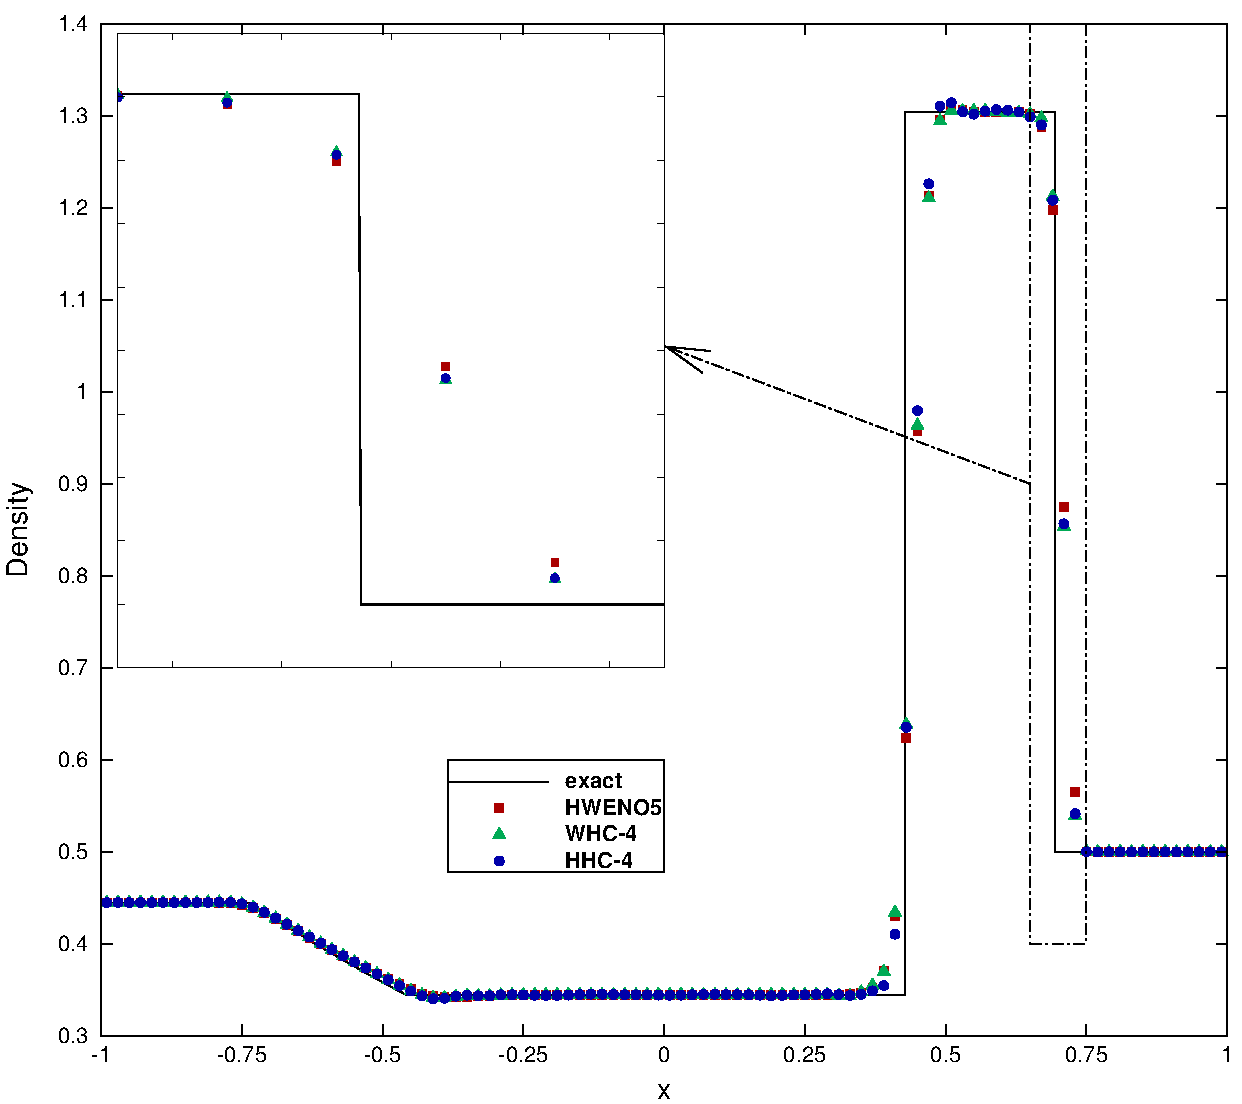
\includegraphics[width=0.75\textwidth]{fig/1D/Ex2.pdf}
  \caption{一维数值格式在\cref{ex:lax} 中密度的图像。
    展示的是$t^{tem} = 0.28$时刻,
    $100$个网格的结果。
  }
  \label{fig:2_1}
\end{figure}

\begin{example}[一维欧拉方程组的Shu-Osher问题]
  \label{ex:osher}
  这个问题最初是由Shu和Osher在文\cite{ShuOsherProblem}中提出的,
  以欧拉方程组 \cref{eq:1D-Euler} 作为模型,
  初值为
  \begin{equation}
    \begin{aligned}
      (\rho,u,p)(x,0)=
      \begin{cases}
        (3.857143,2.629369,10.33333), & x<-4,  \\
        (1 + 0.2\sin(5 x),0,1),       & x>-4.
      \end{cases}
    \end{aligned}
  \end{equation}
\end{example}

在终止时刻$t^{tem}=1.8$,
使用$400$个网格,
采用WHC-4和HHC-4格式计算得到的数值结果见\cref{fig:3_1}。
其中的参考解是GRP格式\upcite{Book-Matania}在$10000$个网格上计算得到的,
\cref{ex:toro,ex:blast-wave} 也是一样的。
我们发现WHC-4格式并不如S2O4-HWENO5格式好。
这是因为高频振荡被WENO类型的非线性权视为间断。
然后,
在高频振荡区域,
WHC-4格式大量使用了二阶重构。
因此,
高频振荡被至多二阶的重构的数值耗散效应磨光了。
在同一区域,
S2O4-HWENO5格式的候选模板的权重不是线性权,
精度降到三阶,
因为其候选模板的精度阶数都是三阶的。
因此,
在这个算例中,
S2O4-HWENO5格式比WHC-4格式做得更好。
HHC-4格式在这个算例中用推荐的$\bar\vartheta$值解决了这个难题。
在高频振荡区域应用了四阶重构。
因此,
我们发现HHC-4格式比S2O4-HWENO5格式稍微好一些。

\begin{figure}[htbp]
  \centering
  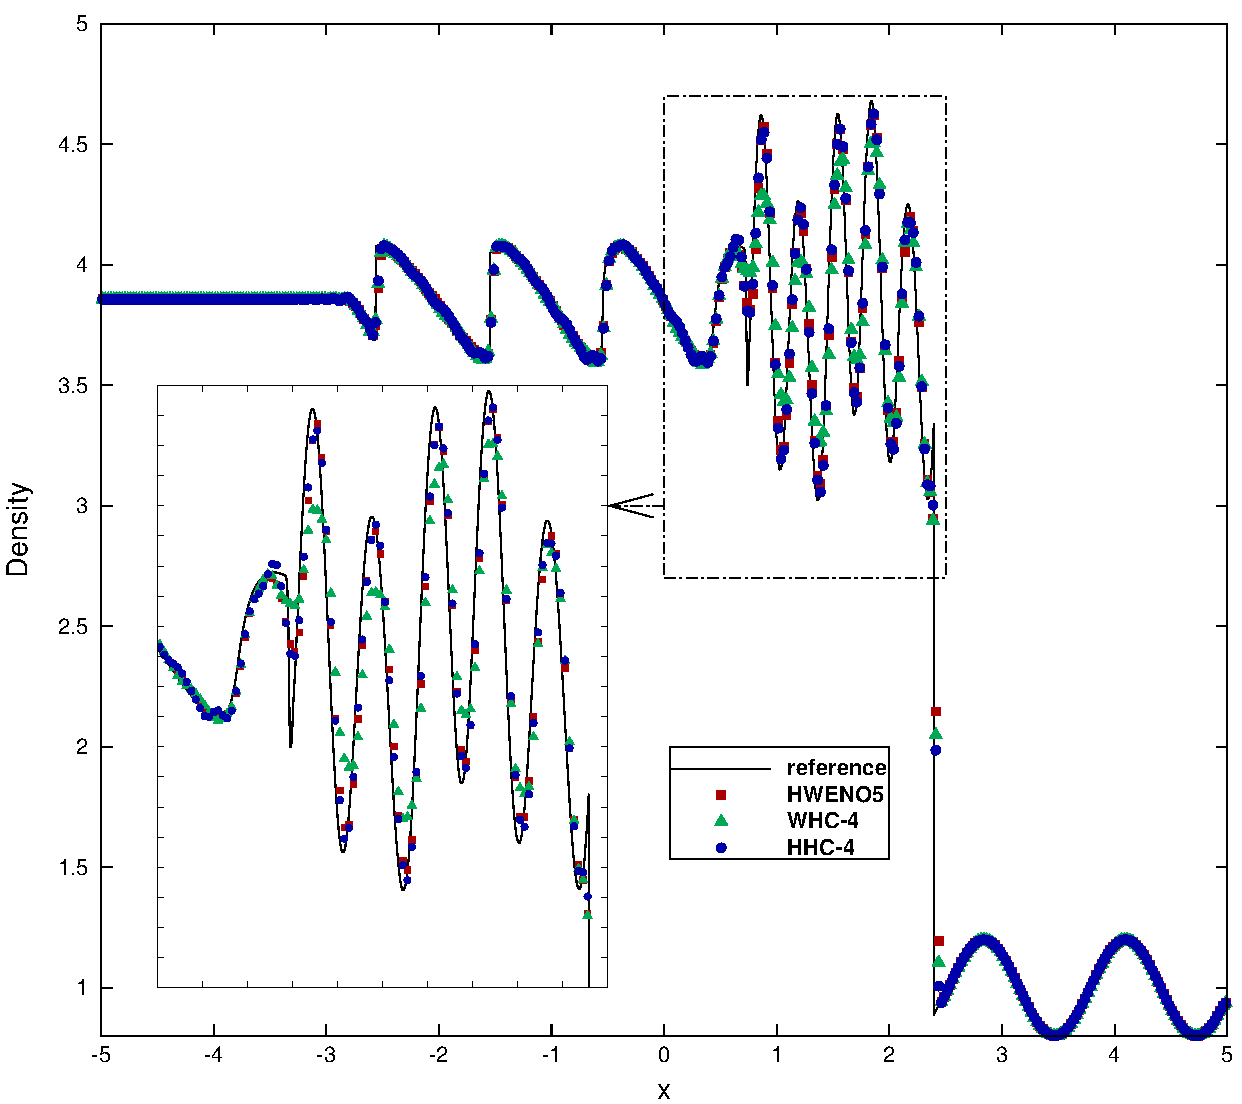
\includegraphics[width=0.75\textwidth]{fig/1D/Ex3.pdf}
  \caption{一维数值格式在\cref{ex:osher} 中密度的图像。
    展示的是$t^{tem} = 1.8$时刻,
    $400$个网格的结果。
  }
  \label{fig:3_1}
\end{figure}

\begin{example}[一维欧拉方程组的Titarev-Toro问题]
  \label{ex:toro}
  这个问题最初是由Titarev和Toro在文\cite{ToroProblem}中提出的,
  以欧拉方程组 \cref{eq:1D-Euler} 作为模型,
  初值为
  \begin{equation}
    \begin{aligned}
      (\rho, u, p)(x,0)=
      \begin{cases}
        (1.515695,0.523346,1.805),  & x<-4.5,  \\
        (1 + 0.1\sin(20\pi x),0,1), & x>-4.5.
      \end{cases}
    \end{aligned}
  \end{equation}
\end{example}

在终止时刻$t^{tem}=5$,
使用$1000$个网格,
采用WHC-4和HHC-4格式计算得到的数值结果见\cref{fig:4_1}。
我们发现数值结果与\cref{ex:osher} 中的结果相似,
HHC-4格式比S2O4-HWENO5格式做得更好。
这里使用了一个较大的值$\bar\vartheta=500$来面对振荡频率更高的问题。
如此做的原因是,
如果$\bar\vartheta$取得较小,
高频振荡会被误认为是间断。

\begin{figure}[htbp]
  \centering
  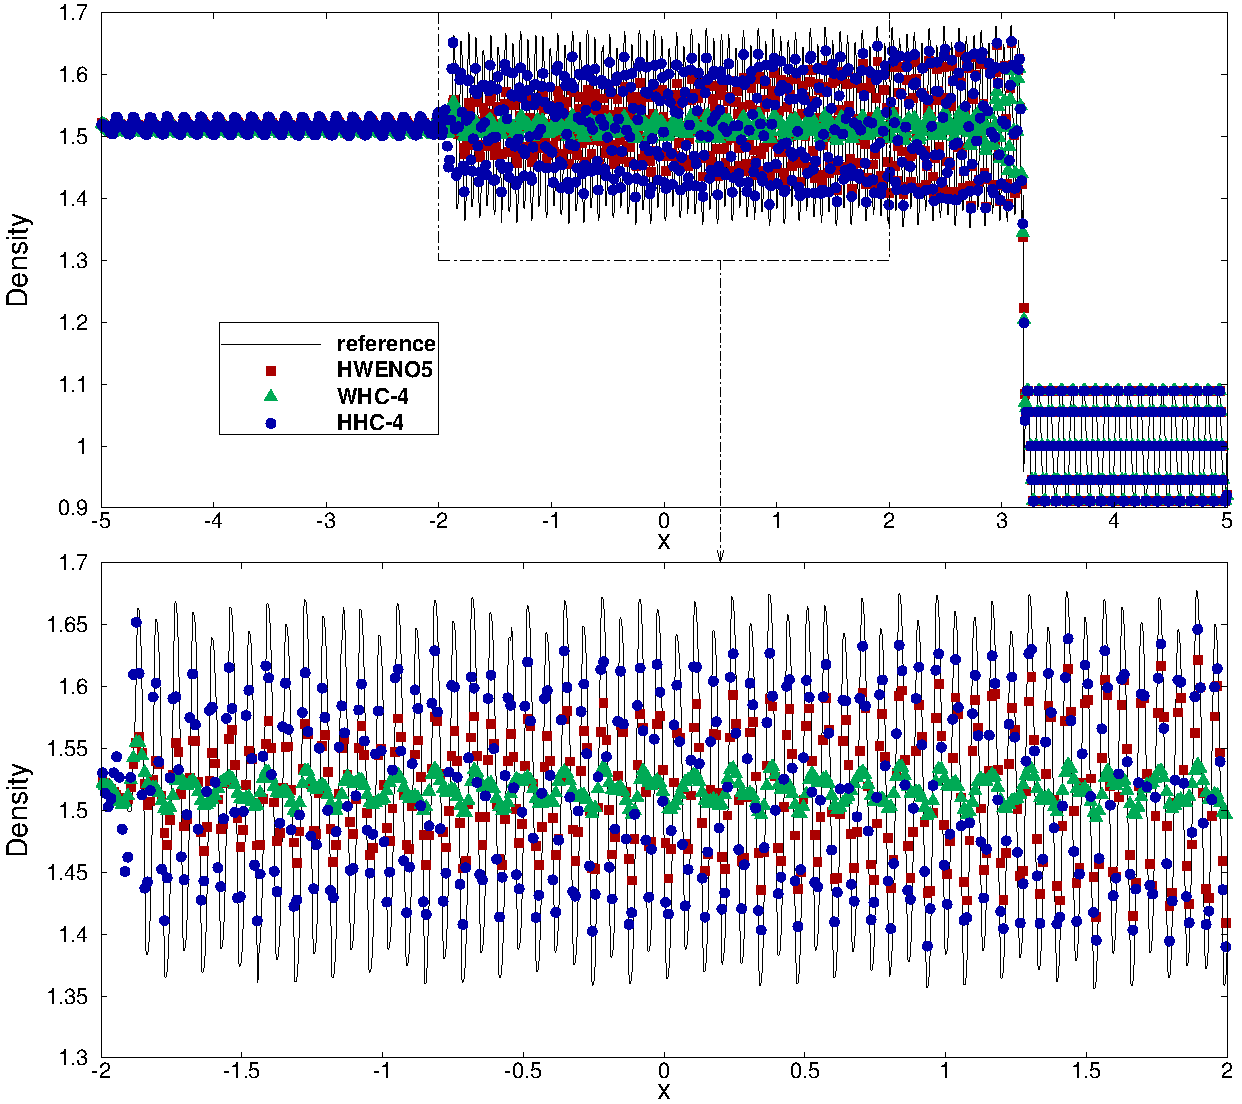
\includegraphics[width=0.75\textwidth]{fig/1D/Ex4.pdf}
  \caption{一维数值格式在\cref{ex:toro} 中密度的图像。
    展示的是$t^{tem} = 5$时刻,
    $1000$个网格的结果。
  }
  \label{fig:4_1}
\end{figure}

\begin{example}[一维欧拉方程组的爆炸波问题]
  \label{ex:blast-wave}
  这个问题最初是由Woodward和Colella在文\cite{frontStep-BlastProblem}中提出的,
  以欧拉方程组 \cref{eq:1D-Euler} 作为模型,
  初值为
  \begin{equation}
    \begin{aligned}
      (\rho,u,p)(x,0)=
      \begin{cases}
        (1,0,10^3),    & x<0.1,     \\
        (1,0,10^{-2}), & 0.1<x<0.9, \\
        (1,0,10^2),    & x>0.9.
      \end{cases}
    \end{aligned}
  \end{equation}
  在计算区域的两侧,
  使用了反射边界条件。
\end{example}

在终止时刻$t^{tem}=0.038$,
使用$300$个网格,
采用WHC-4和HHC-4格式计算得到的数值结果见\cref{fig:5_1}。
WHC-4和HHC-4两种格式都可以很好的捕捉强激波。
从分辨率的角度看,
HHC-4格式最好,
其次是WHC-4格式。

\begin{figure}[htbp]
  \centering
  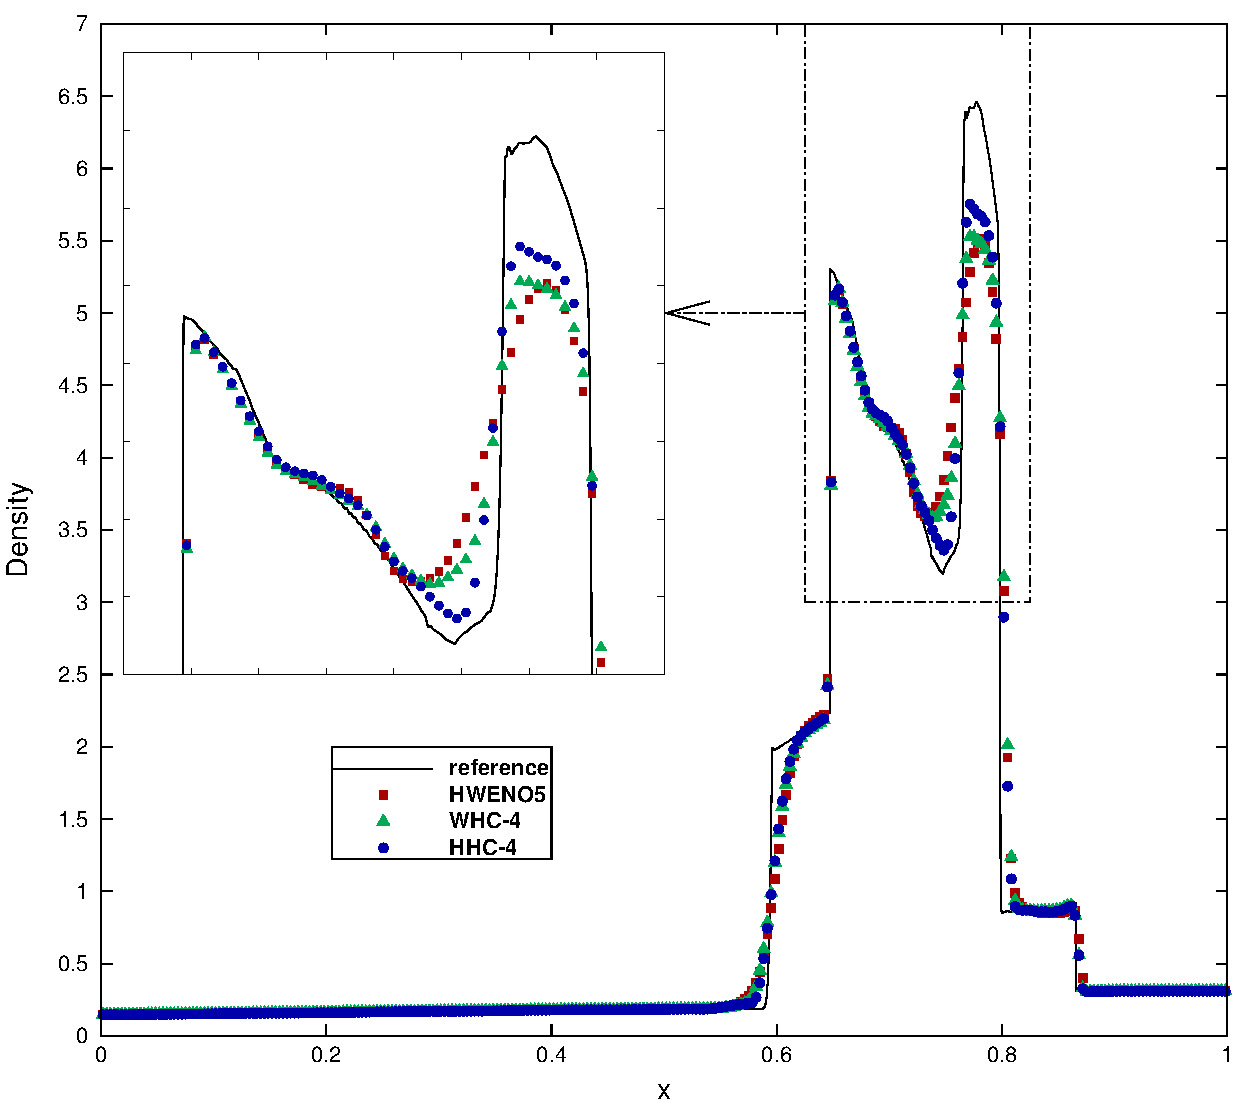
\includegraphics[width=0.75\textwidth]{fig/1D/Ex5.pdf}
  \caption{一维数值格式在\cref{ex:blast-wave} 中密度的图像。
    展示的是$t^{tem} = 0.038$时刻,
    $300$个网格的结果。
  }
  \label{fig:5_1}
\end{figure}

\begin{example}[一维欧拉方程组的大压力/密度比问题]
  \label{ex:large-ratio}
  这个问题最初是由Tang和Liu在文\cite{LPDRP}中提出的,
  以欧拉方程组 \cref{eq:1D-Euler} 作为模型,
  初值为
  \begin{equation}
    \begin{aligned}
      (\rho, u, p)(x,0)=
      \begin{cases}
        (10^4,0,10^4), & x<0.3,  \\
        (1,0,1),       & x>0.3.
      \end{cases}
    \end{aligned}
  \end{equation}
\end{example}

在终止时刻$t^{tem}=0.12$,
使用$300$个网格,
采用WHC-4和HHC-4格式计算得到的数值结果见\cref{fig:6_1}。
这个算例中的CFL数取$0.2$。
WHC-4和HHC-4两种格式都可以比S2O4-HWENO5格式更好地捕捉激波。
HHC-4格式比WHC-4格式稍微好一点。

\begin{figure}[htbp]
  \centering
  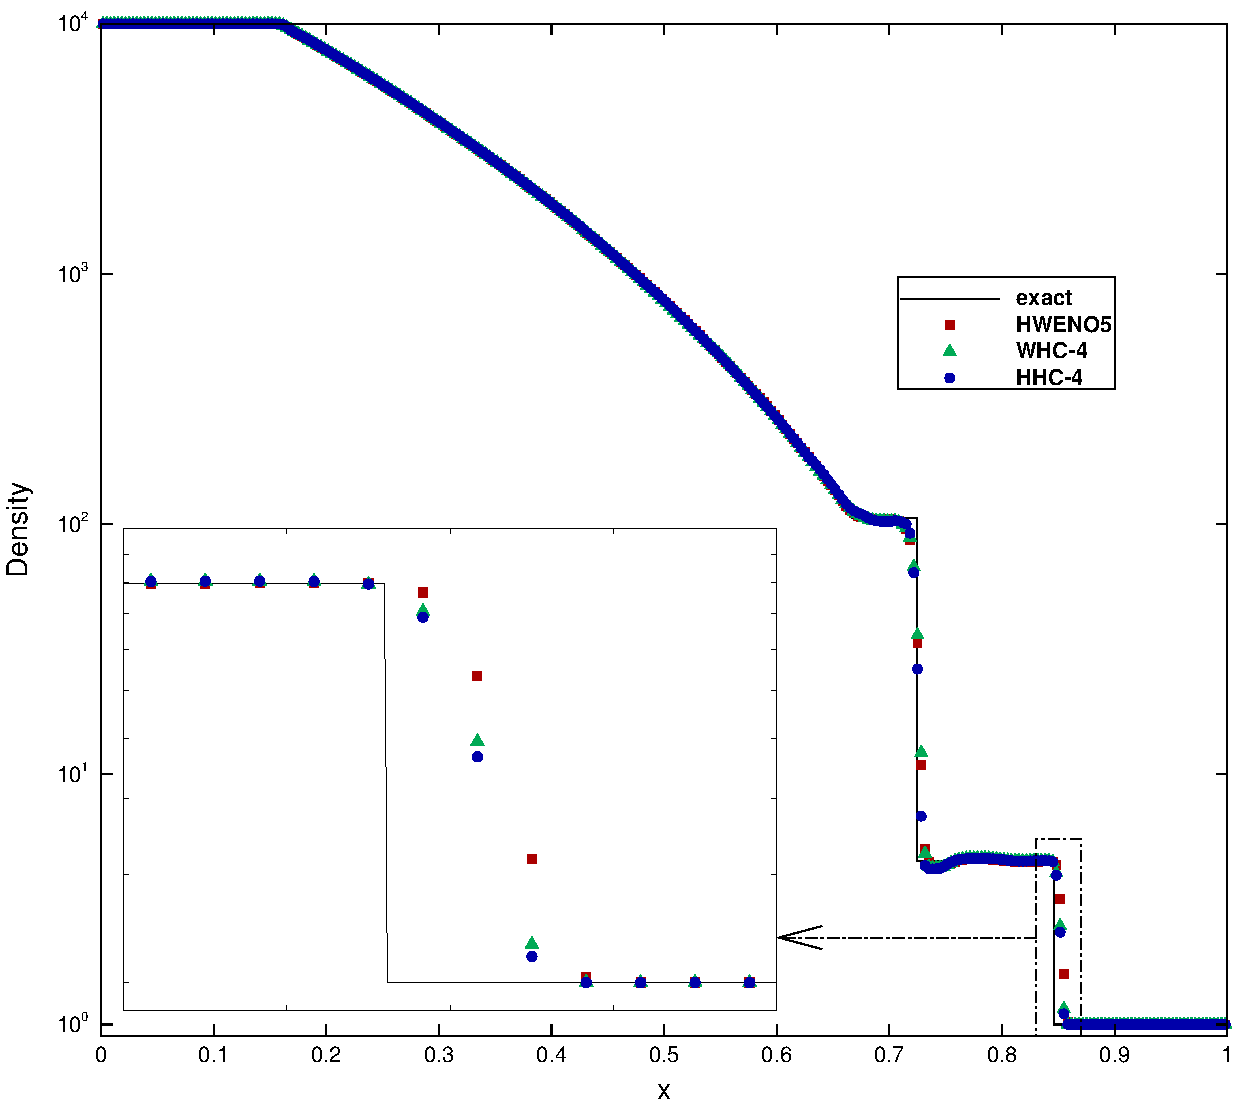
\includegraphics[width=0.75\textwidth]{fig/1D/Ex6.pdf}
  \caption{一维数值格式在\cref{ex:large-ratio} 中密度的图像。
    展示的是$t^{tem} = 0.12$时刻,
    $300$个网格的结果。
  }
  \label{fig:6_1}
\end{figure}

\subsection{空间六阶和八阶精度的两步四阶格式}

接下来,
我们将测试空间六阶和八阶精度的两步四阶格式的数值性能。

\begin{exampleRe}{ex:1D-acc1}{-2}[一维欧拉方程组的精度测试]
  \label{ex:1D-acc1-re}
  这个算例选择线性对流方程 \cref{eq:1D-linear} 作为模型,
  初值为
  \begin{equation}
    u(x, 0) = 1 + 0.2\sin(\pi x).
  \end{equation}
  计算区域是$[-1,1]$,
  采取周期边界条件。
  这个问题的精确解是$u(x,t) = u(x-t,0)$。
\end{exampleRe}

对应于时间$t^{tem}=1$,
采用HC-6、HC-8、WHC-8和HHC-8格式计算得到的变量$u$的单元平均值的误差见\cref{ta:1D-ex1-HC6,ta:1D-ex1-HC8,ta:1D-ex1-WHC8,ta:1D-ex1-HHC8},
其中的“Nstep”代表时间推进的次数。
所有的格式在光滑区域都达到了预期的精度阶数。
其中,
空间六阶和八阶的两步四阶格式采用了\cref{re:high-rec-order} 中的技术来得到重构算法的精度阶数。

\begin{remark}
  \label{re:high-rec-order}
  对于像HC-6和HC-8这样的数值格式,
  它在空间上具有六阶和八阶精度,
  但在时间上只有四阶精度,
  我们不能直接得到重构算法的精度阶数。
  以空间六阶的两步四阶格式为例,
  我们有误差估计
  \begin{equation}
    E(h,C_{CFL}) = \widetilde C_1 \tau^4 + C_2 h^6 = C_1 C_{CFL}^4 h^4 + C_2 h^6,
  \end{equation}
  因此,
  对于相邻的两个单元大小$h$和$h/2$,
  我们分别取CFL数为$c$和$c/\sqrt{2}$,
  那么我们有
  \begin{equation}
    E(h, c) = C_1 c^4 h^4 + C_2 h^6, \quad
    E\left(\frac{h}{2}, \frac{c}{\sqrt{2}}\right) = C_1 \left(\frac{c}{\sqrt{2}}\right)^4 \left(\frac{h}{2}\right)^4 + C_2 \left(\frac{h}{2}\right)^6 = \frac{E(h, c)}{2^6}.
  \end{equation}
  随后,
  通过取$E(h, c)$和$E(h/2, c/\sqrt{2})$的比值并应用对数,
  我们可以得到重构的阶数。
\end{remark}

\def\titleintable{CFL&$h$&Nstep&$L^1$-error&$L^1$-order&$L^\infty$-error&$L^\infty$-order\\}
% \begin{table}[htbp]
% 	\caption{HC-2格式在例 \ref{ex:1D-acc1} 中$u$的$L^1$和$L^\infty$误差和误差阶。展示的是$t^{tem} = 1$时刻的结果。}
% 	\label{ta:1D-ex1-HC2}
% 	\centering
% 	\begin{tabular}{ccccccc}
% 		\toprule
% 		\titleintable
% 		\midrule
% 		0.6 & 2/40   & 34   & 6.36435e-05 &         & 9.97093e-05 &         \\
% 		0.6 & 2/80   & 67   & 1.61841e-05 & \hl{1.97544}& 2.54093e-05 & \hl{1.97237}\\
% 		0.6 & 2/160  & 134  & 4.04954e-06 & \hl{1.99875}& 6.36020e-06 & \hl{1.99821}\\
% 		0.6 & 2/320  & 267  & 1.02222e-06 & \hl{1.98605}& 1.60566e-06 & \hl{1.98591}\\
% 		0.6 & 2/640  & 534  & 2.55932e-07 & \hl{1.99788}& 4.02014e-07 & \hl{1.99785}\\
% 		0.6 & 2/1280 & 1067 & 6.41570e-08 & \hl{1.99608}& 1.00778e-07 & \hl{1.99607}\\
% 		\bottomrule
% 	\end{tabular}
% \end{table}

% \begin{table}[htbp]
% 	\caption{HC-6格式在例 \ref{ex:1D-acc1} 中$u$的$L^1$和$L^\infty$误差和误差阶。展示的是$t^{tem} = 1$时刻的结果。}
% 	\label{ta:1D-ex1-HC6}
% 	\centering
% 	\begin{tabular}{ccccccc}
% 		\toprule
% 		\titleintable
% 		\midrule
% 		0.6   & 2/40  & 34  & 8.91404e-07 &              & 1.40232e-06 &              \\
% 		0.424 & 2/80  & 95  & 2.14939e-08 & \hl{5.37408} & 3.37646e-08 & \hl{5.37616} \\
% 		\midrule
% 		0.6   & 2/80  & 67  & 5.76102e-08 &              & 9.05214e-08 &              \\
% 		0.424 & 2/160 & 189 & 1.35466e-09 & \hl{5.41032} & 2.12794e-09 & \hl{5.41073} \\
% 		\midrule
% 		0.6   & 2/160 & 134 & 3.64358e-09 &              & 5.72373e-09 &              \\
% 		0.424 & 2/320 & 378 & 8.49419e-11 & \hl{5.42274} & 1.33426e-10 & \hl{5.42284} \\
% 		\midrule
% 		0.6   & 2/320 & 267 & 2.29018e-10 &              & 3.59747e-10 &              \\
% 		0.424 & 2/640 & 755 & 5.33039e-12 & \hl{5.42508} & 8.42904e-12 & \hl{5.41547} \\
% 		\bottomrule
% 	\end{tabular}
% \end{table}

% \begin{table}[htbp]
% 	\caption{HC-8格式在例 \ref{ex:1D-acc1} 中$u$的$L^1$和$L^\infty$误差和误差阶。展示的是$t^{tem} = 1$时刻的结果。}
% 	\label{ta:1D-ex1-HC8}
% 	\centering
% 	\begin{tabular}{ccccccc}
% 		\toprule
% 		\titleintable
% 		\midrule
% 		0.6 & 2/20  & 17  & 1.92673e-06 &              & 3.04799e-06 &              \\
% 		0.3 & 2/40  & 67  & 1.34651e-08 & \hl{7.16078} & 2.11098e-08 & \hl{7.17380} \\
% 		\midrule
% 		0.6 & 2/40  & 34  & 1.35577e-07 &              & 2.13057e-07 &              \\
% 		0.3 & 2/80  & 134 & 6.56851e-10 & \hl{7.68933} & 1.03114e-09 & \hl{7.69085} \\
% 		\midrule
% 		0.6 & 2/80  & 67  & 9.04701e-09 &              & 1.42100e-08 &              \\
% 		0.3 & 2/160 & 267 & 3.78187e-11 & \hl{7.90220} & 5.93956e-11 & \hl{7.90233} \\
% 		\midrule
% 		0.6 & 2/160 & 134 & 5.76726e-10 &              & 9.05881e-10 &              \\
% 		0.3 & 2/320 & 534 & 2.31377e-12 & \hl{7.96150} & 3.67661e-12 & \hl{7.94480} \\
% 		\bottomrule
% 	\end{tabular}
% \end{table}

\begin{table}[htbp]
	\caption{WHC-8格式在例 \ref{ex:1D-acc1} 中$u$的$L^1$和$L^\infty$误差和误差阶。展示的是$t^{tem} = 1$时刻的结果。}
	\label{ta:1D-ex1-WHC8}
	\centering
	\begin{tabular}{ccccccc}
		\toprule
		\titleintable
		\midrule
		0.6 & 2/20  & 17  & 1.92673e-06 &              & 3.04799e-06 &              \\
		0.3 & 2/40  & 67  & 1.34651e-08 & \hl{7.16078} & 2.11098e-08 & \hl{7.17380} \\
		\midrule
		0.6 & 2/40  & 34  & 1.35577e-07 &              & 2.13057e-07 &              \\
		0.3 & 2/80  & 134 & 6.56851e-10 & \hl{7.68933} & 1.03114e-09 & \hl{7.69085} \\
		\midrule
		0.6 & 2/80  & 67  & 9.04701e-09 &              & 1.42100e-08 &              \\
		0.3 & 2/160 & 267 & 3.78187e-11 & \hl{7.90220} & 5.93972e-11 & \hl{7.90230} \\
		\midrule
		0.6 & 2/160 & 134 & 5.76726e-10 &              & 9.05879e-10 &              \\
		0.3 & 2/320 & 534 & 2.31375e-12 & \hl{7.96151} & 3.67484e-12 & \hl{7.94549} \\
		\bottomrule
	\end{tabular}
\end{table}

\begin{table}[htbp]
	\caption{HHC-8格式在例 \ref{ex:1D-acc1} 中$u$的$L^1$和$L^\infty$误差和误差阶。展示的是$t^{tem} = 1$时刻的结果。}
	\label{ta:1D-ex1-HHC8}
	\centering
	\begin{tabular}{ccccccc}
		\toprule
		\titleintable
		\midrule
		0.6 & 2/20  & 17  & 1.92673e-06 &              & 3.04799e-06 &              \\
		0.3 & 2/40  & 67  & 1.34651e-08 & \hl{7.16078} & 2.11098e-08 & \hl{7.17380} \\
		\midrule
		0.6 & 2/40  & 34  & 1.35577e-07 &              & 2.13057e-07 &              \\
		0.3 & 2/80  & 134 & 6.56851e-10 & \hl{7.68933} & 1.03114e-09 & \hl{7.69085} \\
		\midrule
		0.6 & 2/80  & 67  & 9.04701e-09 &              & 1.42100e-08 &              \\
		0.3 & 2/160 & 267 & 3.78187e-11 & \hl{7.90220} & 5.93956e-11 & \hl{7.90233} \\
		\midrule
		0.6 & 2/160 & 134 & 5.76726e-10 &              & 9.05881e-10 &              \\
		0.3 & 2/320 & 534 & 2.31377e-12 & \hl{7.96150} & 3.67661e-12 & \hl{7.94480} \\
		\bottomrule
	\end{tabular}
\end{table}
\undef\titleintable

\begin{exampleRe}{ex:1D-acc2}{-2}[一维欧拉方程组的线性退化的精度测试]
  \label{ex:1D-acc2-re}
  此算例以欧拉方程组 \cref{eq:1D-Euler} 作为模型,
  其中多方指数$\gamma$取$1.4$,
  初值为
  \begin{equation}
    \rho(x, 0) = 1 + 0.2\sin(\pi x), \quad u(x,0)=1, \quad p(x,0)=1.
  \end{equation}
  计算区域是$[-1,1]$,
  采取周期边界条件。
  这个问题的精确解是${\bm{u}}(x,t) = {\bm{u}}(x-t,0)$。
\end{exampleRe}

对应于时间$t^{tem}=10$,
采用HC-6、HC-8、WHC-8和HHC-8格式计算得到的密度$\rho$的单元平均值的误差见\cref{ta:1D-ex2-HC6,ta:1D-ex2-HC8,ta:1D-ex2-WHC8,ta:1D-ex2-HHC8},
其中的“Nstep”代表时间推进的次数。
空间八阶的两步四阶格式在光滑区域都达到了预期的精度阶数。
其中,
空间六阶和八阶的两步四阶格式采用了\cref{re:high-rec-order} 中的技术来得到重构算法的精度阶数。
这里的HC-6格式表现出了数值不稳定,
说明这个格式虽然是线性稳定的,
但是应用于非线性方程组时不稳定,
故以后不再使用这个空间六阶的两步四阶格式。

\def\titleintable{CFL&$h$&Nstep&$L^1$-error&$L^1$-order&$L^\infty$-error&$L^\infty$-order\\}
\begin{table}[htbp]
	\caption{HC-6格式在\cref{ex:1D-acc2-re} 中密度的$L^1$和$L^\infty$误差和误差阶。展示的是$t^{tem} = 10$时刻的结果。}
	\label{ta:1D-ex2-HC6}
	\centering
	\begin{tabular}{ccccccc}
		\toprule
		\titleintable
		\midrule
		0.6   & 2/40  & 775   & 8.27459e-07 &          & 1.29667e-06 &          \\
		0.424 & 2/80  & 2190  & 1.86981e-08 & 5.46772  & 2.94233e-08 & 5.46171  \\
		\midrule
		0.6   & 2/80  & 1549  & 5.14263e-08 &          & 8.07340e-08 &          \\
		0.424 & 2/160 & 4381  & 7.21427e-07 & -3.81027 & 2.66267e-06 & -5.04355 \\
		\midrule
		0.6   & 2/160 & 3098  & 7.52045e-09 &          & 2.30543e-08 &          \\
		0.424 & 2/320 & 8761  & 2.90710e-07 & -5.27262 & 8.54718e-07 & -5.21234 \\
		\midrule
		0.6   & 2/320 & 6195  & 3.87887e-07 &          & 1.63360e-06 &          \\
		0.424 & 2/640 & 17521 & 4.45954e-07 & -0.20126 & 1.40088e-06 & 0.22173  \\
		\bottomrule
	\end{tabular}
\end{table}

\begin{table}[htbp]
	\caption{HC-8格式在\cref{ex:1D-acc2-re} 中密度的$L^1$和$L^\infty$误差和误差阶。展示的是$t^{tem} = 10$时刻的结果。}
	\label{ta:1D-ex2-HC8}
	\centering
	\begin{tabular}{ccccccc}
		\toprule
		\titleintable
		\midrule
		0.6 & 20  & 2/387   & 2.30758e-06 &         & 3.64246e-06 &         \\
		0.3 & 40  & 2/1549  & 1.00355e-08 & 7.84513 & 1.57549e-08 & 7.85297 \\
		\midrule
		0.6 & 40  & 2/775   & 8.53015e-08 &         & 1.34196e-07 &         \\
		0.3 & 80  & 2/3098  & 3.59234e-10 & 7.89150 & 5.64030e-10 & 7.89435 \\
		\midrule
		0.6 & 80  & 2/1549  & 3.87437e-09 &         & 6.07971e-09 &         \\
		0.3 & 160 & 2/6195  & 1.56789e-11 & 7.94900 & 2.47085e-11 & 7.94285 \\
		\midrule
		0.6 & 160 & 2/3098  & 2.13053e-10 &         & 3.34755e-10 &         \\
		0.3 & 320 & 2/12389 & 8.64611e-13 & 7.94495 & 1.79901e-12 & 7.53976 \\
		\bottomrule
	\end{tabular}
\end{table}

\begin{table}[htbp]
	\caption{WHC-8格式在\cref{ex:1D-acc2-re} 中密度的$L^1$和$L^\infty$误差和误差阶。展示的是$t^{tem} = 10$时刻的结果。}
	\label{ta:1D-ex2-WHC8}
	\centering
	\begin{tabular}{ccccccc}
		\toprule
		\titleintable
		\midrule
		0.6 & 20  & 2/387   & 2.30758e-06 &         & 3.64246e-06 &         \\
		0.3 & 40  & 2/1549  & 1.00355e-08 & 7.84513 & 1.57549e-08 & 7.85297 \\
		\midrule
		0.6 & 40  & 2/775   & 8.53015e-08 &         & 1.34196e-07 &         \\
		0.3 & 80  & 2/3098  & 3.59238e-10 & 7.89149 & 5.64031e-10 & 7.89435 \\
		\midrule
		0.6 & 80  & 2/1549  & 3.87437e-09 &         & 6.07972e-09 &         \\
		0.3 & 160 & 2/6195  & 1.56794e-11 & 7.94895 & 2.47098e-11 & 7.94278 \\
		\midrule
		0.6 & 160 & 2/3098  & 2.13052e-10 &         & 3.34754e-10 &         \\
		0.3 & 320 & 2/12389 & 8.67489e-13 & 7.94014 & 1.80767e-12 & 7.53283 \\
		\bottomrule
	\end{tabular}
\end{table}

\begin{table}[htbp]
	\caption{HHC-8格式在\cref{ex:1D-acc2-re} 中密度的$L^1$和$L^\infty$误差和误差阶。展示的是$t^{tem} = 10$时刻的结果。}
	\label{ta:1D-ex2-HHC8}
	\centering
	\begin{tabular}{ccccccc}
		\toprule
		\titleintable
		\midrule
		0.6 & 20  & 2/387   & 2.30758e-06 &         & 3.64246e-06 &         \\
		0.3 & 40  & 2/1549  & 1.00355e-08 & 7.84513 & 1.57549e-08 & 7.85297 \\
		\midrule
		0.6 & 40  & 2/775   & 8.53015e-08 &         & 1.34196e-07 &         \\
		0.3 & 80  & 2/3098  & 3.59237e-10 & 7.89149 & 5.64027e-10 & 7.89436 \\
		\midrule
		0.6 & 80  & 2/1549  & 3.87437e-09 &         & 6.07972e-09 &         \\
		0.3 & 160 & 2/6195  & 1.56783e-11 & 7.94905 & 2.47069e-11 & 7.94295 \\
		\midrule
		0.6 & 160 & 2/3098  & 2.13050e-10 &         & 3.34751e-10 &         \\
		0.3 & 320 & 2/12389 & 8.66274e-13 & 7.94215 & 1.80056e-12 & 7.53850 \\
		\bottomrule
	\end{tabular}
\end{table}
\undef\titleintable

\begin{exampleRe}{ex:1D-acc3}{-2}[一维欧拉方程组的非线性的精度测试]
  \label{ex:1D-acc3-re}
  这是一个源自文\cite{Gamma3-HWENO}的数值算例,
  初始条件设定为
  \begin{equation}
    \rho(x, 0)=\frac{1+0.2x}{\sqrt{12}}, \quad
    u(x, 0)=\sqrt{\gamma}\rho(x, y, 0), \quad
    p(x, 0)=\rho(x, 0)^\gamma.
  \end{equation}
  计算区域是$[0, 2\pi]$,
  并且使用与\cref{ex:1D-acc2} 相同的欧拉方程组 \cref{eq:1D-Euler}、均匀网格和周期边界。
  不过,
  多方指数$\gamma$设定为3。
\end{exampleRe}

对应于时间$t^{tem}=3$,
采用HC-8、WHC-8和HHC-8格式计算得到的密度$\rho$的单元平均值的误差见\cref{ta:1D-ex3-HC8,ta:1D-ex3-WHC8,ta:1D-ex3-HHC8},
其中的“Nstep”代表时间推进的次数。
所有的格式在光滑区域都达到了预期的精度阶数,
并采用了\cref{re:high-rec-order} 中的技术来得到重构算法的精度阶数。

\def\titleintable{CFL&$h$&Nstep&$L^1$-error&$L^1$-order&$L^\infty$-error&$L^\infty$-order\\}
% \begin{table}[htbp]
% 	\caption{HC-8格式在例 \ref{ex:1D-acc3} 中密度的$L^1$和$L^\infty$误差和误差阶。展示的是$t^{tem} = 3$时刻的结果。}
% 	\label{ta:1D-ex3-HC8}
% 	\centering
% 	\begin{tabular}{ccccccc}
% 		\toprule
% 		\titleintable
% 		\midrule
% 		0.6 & $2\pi$/80   & 77   & 1.17348e-07 &         & 2.17942e-06 &         \\
% 		0.3 & $2\pi$/160  & 306  & 9.32693e-10 & 6.97518 & 2.03143e-08 & 6.74530 \\
% 		\midrule
% 		0.6 & $2\pi$/160  & 153  & 5.21317e-09 &         & 1.04608e-07 &         \\
% 		0.3 & $2\pi$/320  & 612  & 3.36388e-11 & 7.27589 & 7.47703e-10 & 7.12831 \\
% 		\midrule
% 		0.6 & $2\pi$/320  & 306  & 2.72365e-10 &         & 4.77446e-09 &         \\
% 		0.3 & $2\pi$/640  & 1223 & 1.39036e-12 & 7.61394 & 2.82590e-11 & 7.40048 \\
% 		\midrule
% 		0.6 & $2\pi$/640  & 612  & 1.63513e-11 &         & 2.68696e-10 &         \\
% 		0.3 & $2\pi$/1280 & 2445 & 9.85380e-14 & 7.37451 & 1.33188e-12 & 7.65637 \\
% 		\bottomrule
% 	\end{tabular}
% \end{table}

\begin{table}[htbp]
	% \caption{WHC-8格式在例 \ref{ex:1D-acc3} 中密度的$L^1$和$L^\infty$误差和误差阶。展示的是$t^{tem} = 3$时刻的结果。}
	\label{ta:1D-ex3-WHC8}
	\centering
	\begin{tabular}{ccccccc}
		\toprule
		\titleintable
		\midrule
		0.6 & $2\pi$/80   & 77   & 1.17348e-07 &              & 2.17942e-06 &              \\
		0.3 & $2\pi$/160  & 306  & 9.32693e-10 & \hl{6.97518} & 2.03143e-08 & \hl{6.74530} \\
		\midrule
		0.6 & $2\pi$/160  & 153  & 5.21317e-09 &              & 1.04608e-07 &              \\
		0.3 & $2\pi$/320  & 612  & 3.36388e-11 & \hl{7.27589} & 7.47703e-10 & \hl{7.12831} \\
		\midrule
		0.6 & $2\pi$/320  & 306  & 2.72365e-10 &              & 4.77446e-09 &              \\
		0.3 & $2\pi$/640  & 1223 & 1.39030e-12 & \hl{7.61400} & 2.82586e-11 & \hl{7.40050} \\
		\midrule
		0.6 & $2\pi$/640  & 612  & 1.63512e-11 &              & 2.68696e-10 &              \\
		0.3 & $2\pi$/1280 & 2445 & 9.84114e-14 & \hl{7.37636} & 1.33077e-12 & \hl{7.65757} \\
		\bottomrule
	\end{tabular}
\end{table}

\begin{table}[htbp]
	% \caption{HHC-8格式在例 \ref{ex:1D-acc3} 中密度的$L^1$和$L^\infty$误差和误差阶。展示的是$t^{tem} = 3$时刻的结果。}
	\label{ta:1D-ex3-HHC8}
	\centering
	\begin{tabular}{ccccccc}
		\toprule
		\titleintable
		\midrule
		0.6 & $2\pi$/80   & 77   & 1.17348e-07 &              & 2.17942e-06 &              \\
		0.3 & $2\pi$/160  & 306  & 9.32693e-10 & \hl{6.97518} & 2.03143e-08 & \hl{6.74530} \\
		\midrule
		0.6 & $2\pi$/160  & 153  & 5.21317e-09 &              & 1.04608e-07 &              \\
		0.3 & $2\pi$/320  & 612  & 3.36388e-11 & \hl{7.27589} & 7.47703e-10 & \hl{7.12831} \\
		\midrule
		0.6 & $2\pi$/320  & 306  & 2.72365e-10 &              & 4.77446e-09 &              \\
		0.3 & $2\pi$/640  & 1223 & 1.39036e-12 & \hl{7.61394} & 2.82580e-11 & \hl{7.40054} \\
		\midrule
		0.6 & $2\pi$/640  & 612  & 1.63512e-11 &              & 2.68697e-10 &              \\
		0.3 & $2\pi$/1280 & 2445 & 9.84530e-14 & \hl{7.37575} & 1.33171e-12 & \hl{7.65655} \\
		\bottomrule
	\end{tabular}
\end{table}
\undef\titleintable

\subsection{数值格式的时间效率}

在比较空间四阶和八阶的两步四阶格式时,
我们应该关注在相同的误差下哪个格式的计算时间(CPU时间)更短。
如\cref{fig:1D-time} 所示,
我们可以观察到空间八阶的两步四阶格式展现出了更优的时间效率。

\begin{figure}[htbp]
  \centering
  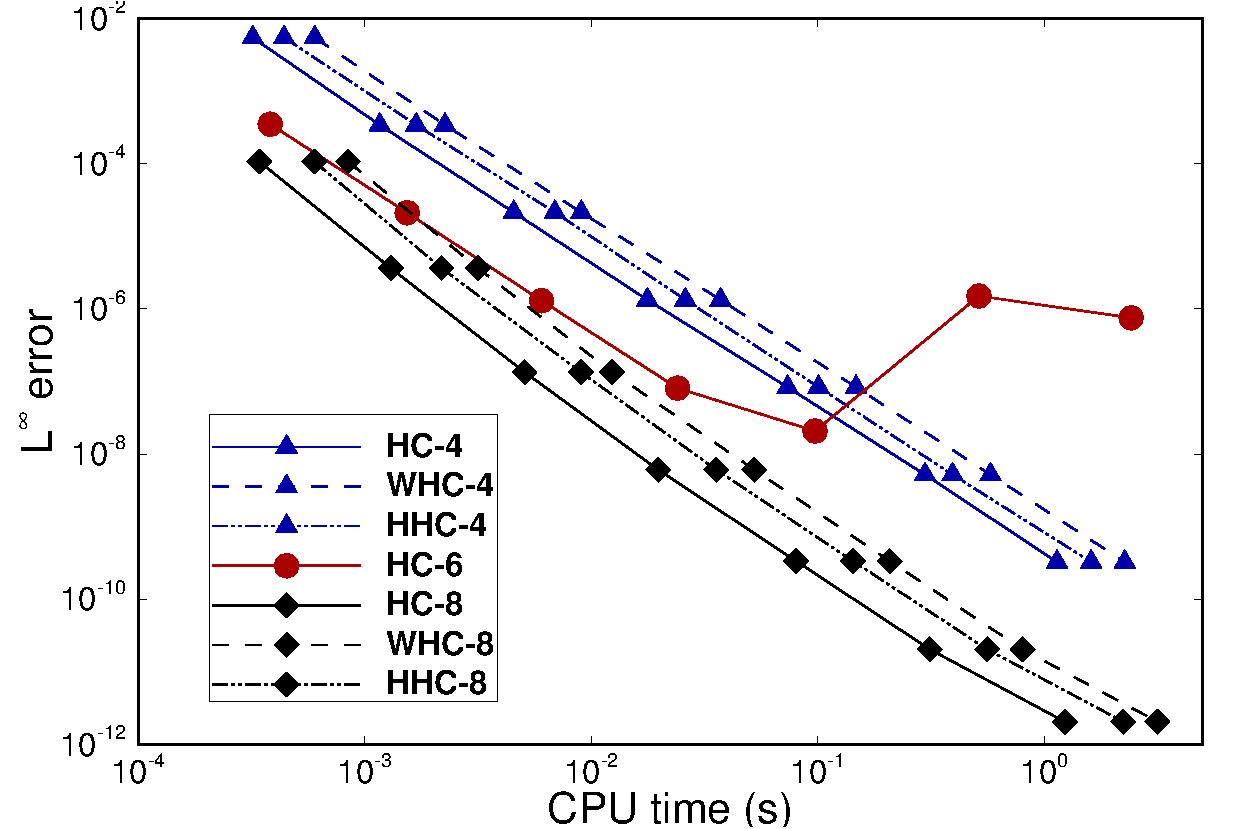
\includegraphics[width=0.8\textwidth]{fig/Time/Time-1D.pdf}
  \caption{几种数值格式在\cref{ex:1D-acc2-re} 中CPU时间与密度的$L^\infty$误差之间的关系。
  }
  \label{fig:1D-time}
\end{figure}

\section{小结}

本章针对一维双曲守恒律,
设计了基于紧致埃尔米特重构的两步四阶数值格式。
具体来说,
我们先构造了不同精度的线性埃尔米特重构,
并设计了相应的线性格式。
然后,
我们做了线性稳定性分析,
在空间四阶、六阶和八阶精度下,
分别得到了一个线性稳定的两步四阶数值格式。
接着,
我们构造了两种四阶精度基本无振荡的非线性重构,
即加权型和杂交选择型的紧致埃尔米特重构,
并设计了相应的时空四阶精度基本无振荡的两步四阶格式。
两种格式均采用Godunov解法器和广义黎曼问题解法器。
我们也将格式推广到了空间八阶精度。
过后,
我们讨论了数值格式的紧致性,
得出了结论:与文\cite{du2018hermite}中的一维两步四阶格式相比,
我们的一维四阶精度两步四阶格式更加紧致。
最后我们给出了许多算例,
验证了我们的数值格式具有高精度、稳定、紧致、高效以及基本无振荡的优良特性。